\documentclass[]{book}
\usepackage{lmodern}
\usepackage{amssymb,amsmath}
\usepackage{ifxetex,ifluatex}
\usepackage{fixltx2e} % provides \textsubscript
\ifnum 0\ifxetex 1\fi\ifluatex 1\fi=0 % if pdftex
  \usepackage[T1]{fontenc}
  \usepackage[utf8]{inputenc}
\else % if luatex or xelatex
  \ifxetex
    \usepackage{mathspec}
  \else
    \usepackage{fontspec}
  \fi
  \defaultfontfeatures{Ligatures=TeX,Scale=MatchLowercase}
\fi
% use upquote if available, for straight quotes in verbatim environments
\IfFileExists{upquote.sty}{\usepackage{upquote}}{}
% use microtype if available
\IfFileExists{microtype.sty}{%
\usepackage{microtype}
\UseMicrotypeSet[protrusion]{basicmath} % disable protrusion for tt fonts
}{}
\usepackage[margin=1in]{geometry}
\usepackage{hyperref}
\hypersetup{unicode=true,
            pdftitle={R Code for Mastering 'Metrics},
            pdfauthor={Jeffrey B. Arnold},
            pdfborder={0 0 0},
            breaklinks=true}
\urlstyle{same}  % don't use monospace font for urls
\usepackage{color}
\usepackage{fancyvrb}
\newcommand{\VerbBar}{|}
\newcommand{\VERB}{\Verb[commandchars=\\\{\}]}
\DefineVerbatimEnvironment{Highlighting}{Verbatim}{commandchars=\\\{\}}
% Add ',fontsize=\small' for more characters per line
\usepackage{framed}
\definecolor{shadecolor}{RGB}{248,248,248}
\newenvironment{Shaded}{\begin{snugshade}}{\end{snugshade}}
\newcommand{\AlertTok}[1]{\textcolor[rgb]{0.94,0.16,0.16}{#1}}
\newcommand{\AnnotationTok}[1]{\textcolor[rgb]{0.56,0.35,0.01}{\textbf{\textit{#1}}}}
\newcommand{\AttributeTok}[1]{\textcolor[rgb]{0.77,0.63,0.00}{#1}}
\newcommand{\BaseNTok}[1]{\textcolor[rgb]{0.00,0.00,0.81}{#1}}
\newcommand{\BuiltInTok}[1]{#1}
\newcommand{\CharTok}[1]{\textcolor[rgb]{0.31,0.60,0.02}{#1}}
\newcommand{\CommentTok}[1]{\textcolor[rgb]{0.56,0.35,0.01}{\textit{#1}}}
\newcommand{\CommentVarTok}[1]{\textcolor[rgb]{0.56,0.35,0.01}{\textbf{\textit{#1}}}}
\newcommand{\ConstantTok}[1]{\textcolor[rgb]{0.00,0.00,0.00}{#1}}
\newcommand{\ControlFlowTok}[1]{\textcolor[rgb]{0.13,0.29,0.53}{\textbf{#1}}}
\newcommand{\DataTypeTok}[1]{\textcolor[rgb]{0.13,0.29,0.53}{#1}}
\newcommand{\DecValTok}[1]{\textcolor[rgb]{0.00,0.00,0.81}{#1}}
\newcommand{\DocumentationTok}[1]{\textcolor[rgb]{0.56,0.35,0.01}{\textbf{\textit{#1}}}}
\newcommand{\ErrorTok}[1]{\textcolor[rgb]{0.64,0.00,0.00}{\textbf{#1}}}
\newcommand{\ExtensionTok}[1]{#1}
\newcommand{\FloatTok}[1]{\textcolor[rgb]{0.00,0.00,0.81}{#1}}
\newcommand{\FunctionTok}[1]{\textcolor[rgb]{0.00,0.00,0.00}{#1}}
\newcommand{\ImportTok}[1]{#1}
\newcommand{\InformationTok}[1]{\textcolor[rgb]{0.56,0.35,0.01}{\textbf{\textit{#1}}}}
\newcommand{\KeywordTok}[1]{\textcolor[rgb]{0.13,0.29,0.53}{\textbf{#1}}}
\newcommand{\NormalTok}[1]{#1}
\newcommand{\OperatorTok}[1]{\textcolor[rgb]{0.81,0.36,0.00}{\textbf{#1}}}
\newcommand{\OtherTok}[1]{\textcolor[rgb]{0.56,0.35,0.01}{#1}}
\newcommand{\PreprocessorTok}[1]{\textcolor[rgb]{0.56,0.35,0.01}{\textit{#1}}}
\newcommand{\RegionMarkerTok}[1]{#1}
\newcommand{\SpecialCharTok}[1]{\textcolor[rgb]{0.00,0.00,0.00}{#1}}
\newcommand{\SpecialStringTok}[1]{\textcolor[rgb]{0.31,0.60,0.02}{#1}}
\newcommand{\StringTok}[1]{\textcolor[rgb]{0.31,0.60,0.02}{#1}}
\newcommand{\VariableTok}[1]{\textcolor[rgb]{0.00,0.00,0.00}{#1}}
\newcommand{\VerbatimStringTok}[1]{\textcolor[rgb]{0.31,0.60,0.02}{#1}}
\newcommand{\WarningTok}[1]{\textcolor[rgb]{0.56,0.35,0.01}{\textbf{\textit{#1}}}}
\usepackage{longtable,booktabs}
\usepackage{graphicx,grffile}
\makeatletter
\def\maxwidth{\ifdim\Gin@nat@width>\linewidth\linewidth\else\Gin@nat@width\fi}
\def\maxheight{\ifdim\Gin@nat@height>\textheight\textheight\else\Gin@nat@height\fi}
\makeatother
% Scale images if necessary, so that they will not overflow the page
% margins by default, and it is still possible to overwrite the defaults
% using explicit options in \includegraphics[width, height, ...]{}
\setkeys{Gin}{width=\maxwidth,height=\maxheight,keepaspectratio}
\IfFileExists{parskip.sty}{%
\usepackage{parskip}
}{% else
\setlength{\parindent}{0pt}
\setlength{\parskip}{6pt plus 2pt minus 1pt}
}
\setlength{\emergencystretch}{3em}  % prevent overfull lines
\providecommand{\tightlist}{%
  \setlength{\itemsep}{0pt}\setlength{\parskip}{0pt}}
\setcounter{secnumdepth}{5}
% Redefines (sub)paragraphs to behave more like sections
\ifx\paragraph\undefined\else
\let\oldparagraph\paragraph
\renewcommand{\paragraph}[1]{\oldparagraph{#1}\mbox{}}
\fi
\ifx\subparagraph\undefined\else
\let\oldsubparagraph\subparagraph
\renewcommand{\subparagraph}[1]{\oldsubparagraph{#1}\mbox{}}
\fi

%%% Use protect on footnotes to avoid problems with footnotes in titles
\let\rmarkdownfootnote\footnote%
\def\footnote{\protect\rmarkdownfootnote}

%%% Change title format to be more compact
\usepackage{titling}

% Create subtitle command for use in maketitle
\newcommand{\subtitle}[1]{
  \posttitle{
    \begin{center}\large#1\end{center}
    }
}

\setlength{\droptitle}{-2em}
  \title{R Code for Mastering 'Metrics}
  \pretitle{\vspace{\droptitle}\centering\huge}
  \posttitle{\par}
  \author{Jeffrey B. Arnold}
  \preauthor{\centering\large\emph}
  \postauthor{\par}
  \date{}
  \predate{}\postdate{}


\usepackage{amsthm}
\newtheorem{theorem}{Theorem}[chapter]
\newtheorem{lemma}{Lemma}[chapter]
\newtheorem{corollary}{Corollary}[chapter]
\newtheorem{proposition}{Proposition}[chapter]
\newtheorem{conjecture}{Conjecture}[chapter]
\theoremstyle{definition}
\newtheorem{definition}{Definition}[chapter]
\theoremstyle{definition}
\newtheorem{example}{Example}[chapter]
\theoremstyle{definition}
\newtheorem{exercise}{Exercise}[chapter]
\theoremstyle{remark}
\newtheorem*{remark}{Remark}
\newtheorem*{solution}{Solution}
\begin{document}
\maketitle

{
\setcounter{tocdepth}{1}
\tableofcontents
}
\hypertarget{welcome}{%
\chapter*{Welcome}\label{welcome}}
\addcontentsline{toc}{chapter}{Welcome}

This work contains R code to reproduce many of the analyses in
\emph{Mastering 'Metrics} by Joshua D. Angrist and Jörn-Steffen Pischke
(Angrist and Pischke 2014). This work provides R translations of the
replication code available at
\href{http://masteringmetrics.com/resources/}{masteringmetrics.com}.

The R code used in the examples heavily depends on
\href{https://www.tidyverse.org/}{tidyverse} packages. I suggest
starting with Grolemund and Wickham, \href{http://r4ds.had.co.nz/}{R for
Data Science} if you are unfamiliar with the tidyverse.

\hypertarget{install}{%
\section*{Install}\label{install}}
\addcontentsline{toc}{section}{Install}

To install all R packages and datasets needed to run the examples in
\emph{Mastering 'Metrics} run:

\begin{Shaded}
\begin{Highlighting}[]
\CommentTok{# install.packages("devtools")}
\NormalTok{devtools}\OperatorTok{::}\KeywordTok{install_github}\NormalTok{(}\StringTok{"jrnold/masteringmetrics"}\NormalTok{, }\DataTypeTok{subdir =} \StringTok{"masteringmetrics"}\NormalTok{)}
\end{Highlighting}
\end{Shaded}

\hypertarget{license}{%
\section*{License}\label{license}}
\addcontentsline{toc}{section}{License}

The text of this work is licensed under the
\href{http://creativecommons.org/licenses/by/4.0/}{Creative Commons
Attribution 4.0 International License}. The R Code in this work is
licensed under the \href{https://opensource.org/licenses/MIT}{MIT
License}.

\hypertarget{colonophon}{%
\section*{Colonophon}\label{colonophon}}
\addcontentsline{toc}{section}{Colonophon}

The book is powered by \url{https://bookdown.org} which makes it easy to
turn R markdown files into HTML, PDF, and EPUB.

This book was built with:

\begin{Shaded}
\begin{Highlighting}[]
\NormalTok{devtools}\OperatorTok{::}\KeywordTok{session_info}\NormalTok{(}\KeywordTok{c}\NormalTok{(}\StringTok{"tidyverse"}\NormalTok{))}
\CommentTok{#> Session info -------------------------------------------------------------}
\CommentTok{#>  setting  value                       }
\CommentTok{#>  version  R version 3.4.4 (2018-03-15)}
\CommentTok{#>  system   x86_64, darwin15.6.0        }
\CommentTok{#>  ui       X11                         }
\CommentTok{#>  language (EN)                        }
\CommentTok{#>  collate  en_US.UTF-8                 }
\CommentTok{#>  tz       America/Los_Angeles         }
\CommentTok{#>  date     2018-04-20}
\CommentTok{#> Packages -----------------------------------------------------------------}
\CommentTok{#>  package      * version    date       source                          }
\CommentTok{#>  assertthat     0.2.0      2017-04-11 CRAN (R 3.4.0)                  }
\CommentTok{#>  backports      1.1.2      2017-12-13 CRAN (R 3.4.3)                  }
\CommentTok{#>  base64enc      0.1-3      2015-07-28 CRAN (R 3.4.0)                  }
\CommentTok{#>  BH             1.66.0-1   2018-02-13 CRAN (R 3.4.3)                  }
\CommentTok{#>  bindr          0.1.1      2018-03-13 CRAN (R 3.4.4)                  }
\CommentTok{#>  bindrcpp       0.2.2      2018-03-29 CRAN (R 3.4.4)                  }
\CommentTok{#>  broom          0.4.4      2018-03-29 cran (@0.4.4)                   }
\CommentTok{#>  callr          2.0.3      2018-04-11 cran (@2.0.3)                   }
\CommentTok{#>  cellranger     1.1.0      2016-07-27 CRAN (R 3.4.0)                  }
\CommentTok{#>  cli            1.0.0      2017-11-05 cran (@1.0.0)                   }
\CommentTok{#>  colorspace     1.3-2      2016-12-14 CRAN (R 3.4.0)                  }
\CommentTok{#>  compiler       3.4.4      2018-03-15 local                           }
\CommentTok{#>  crayon         1.3.4      2017-09-16 CRAN (R 3.4.1)                  }
\CommentTok{#>  curl           3.2        2018-03-28 CRAN (R 3.4.4)                  }
\CommentTok{#>  DBI            0.8        2018-03-02 CRAN (R 3.4.3)                  }
\CommentTok{#>  dbplyr         1.2.1      2018-02-19 CRAN (R 3.4.3)                  }
\CommentTok{#>  debugme        1.1.0      2017-10-22 CRAN (R 3.4.2)                  }
\CommentTok{#>  dichromat      2.0-0      2013-01-24 CRAN (R 3.4.0)                  }
\CommentTok{#>  digest         0.6.15     2018-01-28 CRAN (R 3.4.3)                  }
\CommentTok{#>  dplyr          0.7.4      2017-09-28 CRAN (R 3.4.2)                  }
\CommentTok{#>  evaluate       0.10.1     2017-06-24 CRAN (R 3.4.1)                  }
\CommentTok{#>  forcats        0.3.0      2018-02-19 CRAN (R 3.4.3)                  }
\CommentTok{#>  foreign        0.8-69     2017-06-22 CRAN (R 3.4.4)                  }
\CommentTok{#>  ggplot2        2.2.1      2016-12-30 CRAN (R 3.4.0)                  }
\CommentTok{#>  glue           1.2.0      2017-10-29 CRAN (R 3.4.2)                  }
\CommentTok{#>  graphics     * 3.4.4      2018-03-15 local                           }
\CommentTok{#>  grDevices    * 3.4.4      2018-03-15 local                           }
\CommentTok{#>  grid           3.4.4      2018-03-15 local                           }
\CommentTok{#>  gtable         0.2.0      2016-02-26 CRAN (R 3.4.0)                  }
\CommentTok{#>  haven          1.1.1.9000 2018-03-31 Github (tidyverse/haven@746eb3e)}
\CommentTok{#>  highr          0.6        2016-05-09 CRAN (R 3.4.0)                  }
\CommentTok{#>  hms            0.4.2      2018-03-10 CRAN (R 3.4.4)                  }
\CommentTok{#>  htmltools      0.3.6      2017-04-28 CRAN (R 3.4.0)                  }
\CommentTok{#>  httr           1.3.1      2017-08-20 CRAN (R 3.4.1)                  }
\CommentTok{#>  jsonlite       1.5        2017-06-01 CRAN (R 3.4.0)                  }
\CommentTok{#>  knitr          1.20       2018-02-20 CRAN (R 3.4.3)                  }
\CommentTok{#>  labeling       0.3        2014-08-23 CRAN (R 3.4.0)                  }
\CommentTok{#>  lattice        0.20-35    2017-03-25 CRAN (R 3.4.4)                  }
\CommentTok{#>  lazyeval       0.2.1      2017-10-29 CRAN (R 3.4.2)                  }
\CommentTok{#>  lubridate      1.7.4      2018-04-11 CRAN (R 3.4.4)                  }
\CommentTok{#>  magrittr       1.5        2014-11-22 CRAN (R 3.4.0)                  }
\CommentTok{#>  markdown       0.8        2017-04-20 CRAN (R 3.4.0)                  }
\CommentTok{#>  MASS           7.3-49     2018-02-23 CRAN (R 3.4.3)                  }
\CommentTok{#>  methods      * 3.4.4      2018-03-15 local                           }
\CommentTok{#>  mime           0.5        2016-07-07 CRAN (R 3.4.0)                  }
\CommentTok{#>  mnormt         1.5-5      2016-10-15 CRAN (R 3.4.0)                  }
\CommentTok{#>  modelr         0.1.1      2017-07-24 CRAN (R 3.4.1)                  }
\CommentTok{#>  munsell        0.4.3      2016-02-13 CRAN (R 3.4.0)                  }
\CommentTok{#>  nlme           3.1-137    2018-04-07 CRAN (R 3.4.4)                  }
\CommentTok{#>  openssl        1.0.1      2018-03-03 CRAN (R 3.4.3)                  }
\CommentTok{#>  parallel       3.4.4      2018-03-15 local                           }
\CommentTok{#>  pillar         1.2.1      2018-02-27 CRAN (R 3.4.3)                  }
\CommentTok{#>  pkgconfig      2.0.1      2017-03-21 CRAN (R 3.4.0)                  }
\CommentTok{#>  plogr          0.2.0      2018-03-25 CRAN (R 3.4.4)                  }
\CommentTok{#>  plyr           1.8.4      2016-06-08 CRAN (R 3.4.0)                  }
\CommentTok{#>  praise         1.0.0      2015-08-11 CRAN (R 3.4.0)                  }
\CommentTok{#>  psych          1.8.3.3    2018-03-30 CRAN (R 3.4.4)                  }
\CommentTok{#>  purrr          0.2.4      2017-10-18 cran (@0.2.4)                   }
\CommentTok{#>  R6             2.2.2      2017-06-17 CRAN (R 3.4.0)                  }
\CommentTok{#>  RColorBrewer   1.1-2      2014-12-07 CRAN (R 3.4.0)                  }
\CommentTok{#>  Rcpp           0.12.16    2018-03-13 cran (@0.12.16)                 }
\CommentTok{#>  readr          1.1.1      2017-05-16 CRAN (R 3.4.0)                  }
\CommentTok{#>  readxl         1.0.0      2017-04-18 CRAN (R 3.4.0)                  }
\CommentTok{#>  rematch        1.0.1      2016-04-21 CRAN (R 3.4.0)                  }
\CommentTok{#>  reprex         0.1.2      2018-01-26 CRAN (R 3.4.3)                  }
\CommentTok{#>  reshape2       1.4.3      2017-12-11 CRAN (R 3.4.3)                  }
\CommentTok{#>  rlang          0.2.0      2018-02-20 CRAN (R 3.4.3)                  }
\CommentTok{#>  rmarkdown      1.9        2018-03-01 CRAN (R 3.4.3)                  }
\CommentTok{#>  rprojroot      1.3-2      2018-01-03 CRAN (R 3.4.3)                  }
\CommentTok{#>  rstudioapi     0.7        2017-09-07 CRAN (R 3.4.1)                  }
\CommentTok{#>  rvest          0.3.2      2016-06-17 CRAN (R 3.4.0)                  }
\CommentTok{#>  scales         0.5.0      2017-08-24 CRAN (R 3.4.1)                  }
\CommentTok{#>  selectr        0.4-1      2018-04-06 CRAN (R 3.4.4)                  }
\CommentTok{#>  stats        * 3.4.4      2018-03-15 local                           }
\CommentTok{#>  stringi        1.1.7      2018-03-12 CRAN (R 3.4.4)                  }
\CommentTok{#>  stringr        1.3.0      2018-02-19 CRAN (R 3.4.3)                  }
\CommentTok{#>  testthat       2.0.0      2017-12-13 CRAN (R 3.4.3)                  }
\CommentTok{#>  tibble         1.4.2      2018-01-22 CRAN (R 3.4.3)                  }
\CommentTok{#>  tidyr          0.8.0      2018-01-29 CRAN (R 3.4.3)                  }
\CommentTok{#>  tidyselect     0.2.4      2018-02-26 CRAN (R 3.4.3)                  }
\CommentTok{#>  tidyverse      1.2.1      2017-11-14 CRAN (R 3.4.2)                  }
\CommentTok{#>  tools          3.4.4      2018-03-15 local                           }
\CommentTok{#>  utf8           1.1.3      2018-01-03 CRAN (R 3.4.3)                  }
\CommentTok{#>  utils        * 3.4.4      2018-03-15 local                           }
\CommentTok{#>  viridisLite    0.3.0      2018-02-01 CRAN (R 3.4.3)                  }
\CommentTok{#>  whisker        0.3-2      2013-04-28 CRAN (R 3.4.0)                  }
\CommentTok{#>  withr          2.1.2      2018-03-15 CRAN (R 3.4.4)                  }
\CommentTok{#>  xml2           1.2.0      2018-01-24 CRAN (R 3.4.3)                  }
\CommentTok{#>  yaml           2.1.18     2018-03-08 cran (@2.1.18)}
\end{Highlighting}
\end{Shaded}

\hypertarget{part-chapter-1}{%
\part{Chapter 1}\label{part-chapter-1}}

\hypertarget{national-health-interview-survey}{%
\chapter{National Health Interview
Survey}\label{national-health-interview-survey}}

This reproduces the analyses in Table 1.1 of Angrist and Pischke (2014).
which compares people with and without health insurance in the 2009
National Health Interview Survey (NHIS).

The code is derived from
\href{http://masteringmetrics.com/wp-content/uploads/2015/01/NHIS2009_hicompare.do}{NHIS2009\_hicompare.do}.

Load the prerequisite packages.

\begin{Shaded}
\begin{Highlighting}[]
\KeywordTok{library}\NormalTok{(}\StringTok{"tidyverse"}\NormalTok{)}
\KeywordTok{library}\NormalTok{(}\StringTok{"magrittr"}\NormalTok{)}
\KeywordTok{library}\NormalTok{(}\StringTok{"haven"}\NormalTok{)}
\end{Highlighting}
\end{Shaded}

Load the data (originally from
\url{http://masteringmetrics.com/wp-content/uploads/2015/01/Data.zip}),
and adjust a few of the columns to account for differences in how Stata
and R store data.

\begin{Shaded}
\begin{Highlighting}[]
\KeywordTok{data}\NormalTok{(}\StringTok{"NHIS2009"}\NormalTok{, }\DataTypeTok{package =} \StringTok{"masteringmetrics"}\NormalTok{)}
\end{Highlighting}
\end{Shaded}

Remove missing values.

\begin{Shaded}
\begin{Highlighting}[]
\NormalTok{NHIS2009 <-}\StringTok{ }\NormalTok{NHIS2009 }\OperatorTok
\StringTok{  }\KeywordTok{filter}\NormalTok{(marradult, perweight }\OperatorTok{!=}\StringTok{ }\DecValTok{0}\NormalTok{) }\OperatorTok
\StringTok{  }\KeywordTok{group_by}\NormalTok{(serial) }\OperatorTok
\StringTok{  }\KeywordTok{mutate}\NormalTok{(}\DataTypeTok{hi_hsb =} \KeywordTok{mean}\NormalTok{(hi_hsb1, }\DataTypeTok{na.rm =} \OtherTok{TRUE}\NormalTok{)) }\OperatorTok
\StringTok{  }\KeywordTok{filter}\NormalTok{(}\OperatorTok{!}\KeywordTok{is.na}\NormalTok{(hi_hsb), }\OperatorTok{!}\KeywordTok{is.na}\NormalTok{(hi)) }\OperatorTok
\StringTok{  }\KeywordTok{mutate}\NormalTok{(}\DataTypeTok{female =} \KeywordTok{sum}\NormalTok{(fml)) }\OperatorTok
\StringTok{  }\KeywordTok{filter}\NormalTok{(female }\OperatorTok{==}\StringTok{ }\DecValTok{1}\NormalTok{) }\OperatorTok
\StringTok{  }\KeywordTok{select}\NormalTok{(}\OperatorTok{-}\NormalTok{female)}
\end{Highlighting}
\end{Shaded}

For the sample only include married adults between 26 and 59 in age, and
remove single person households.

\begin{Shaded}
\begin{Highlighting}[]
\NormalTok{NHIS2009 <-}\StringTok{ }\NormalTok{NHIS2009 }\OperatorTok
\StringTok{  }\KeywordTok{filter}\NormalTok{(}\KeywordTok{between}\NormalTok{(age, }\DecValTok{26}\NormalTok{, }\DecValTok{59}\NormalTok{),}
\NormalTok{         marradult, adltempl }\OperatorTok{>=}\StringTok{ }\DecValTok{1}\NormalTok{)}
\end{Highlighting}
\end{Shaded}

Keep only single family households.

\begin{Shaded}
\begin{Highlighting}[]
\NormalTok{NHIS2009 <-}\StringTok{ }\NormalTok{NHIS2009 }\OperatorTok
\StringTok{  }\KeywordTok{group_by}\NormalTok{(serial) }\OperatorTok
\StringTok{  }\KeywordTok{filter}\NormalTok{(}\KeywordTok{length}\NormalTok{(serial) }\OperatorTok{>}\StringTok{ }\NormalTok{1L) }\OperatorTok
\StringTok{  }\KeywordTok{ungroup}\NormalTok{()}
\end{Highlighting}
\end{Shaded}

Tables of wives and husbands by health insurance. status. The weighting
following the ``analytic'' weights in the original \texttt{.do} file
which weights observations by \texttt{perweight} and normalizes the
weights so that the sub-samples of males and females have the same
number as the original sample.

\begin{Shaded}
\begin{Highlighting}[]
\NormalTok{NHIS2009 }\OperatorTok
\StringTok{  }\KeywordTok{group_by}\NormalTok{(fml) }\OperatorTok
\StringTok{  }\CommentTok{# normalize person weights to match number of observations in each}
\StringTok{  }\CommentTok{# group}
\StringTok{  }\KeywordTok{mutate}\NormalTok{(}\DataTypeTok{perweight =}\NormalTok{ perweight }\OperatorTok{/}\StringTok{ }\KeywordTok{sum}\NormalTok{(perweight) }\OperatorTok{*}\StringTok{ }\KeywordTok{n}\NormalTok{()) }\OperatorTok
\StringTok{  }\KeywordTok{group_by}\NormalTok{(fml, hi) }\OperatorTok
\StringTok{  }\KeywordTok{summarise}\NormalTok{(}\DataTypeTok{n_wt =} \KeywordTok{sum}\NormalTok{(perweight)) }\OperatorTok
\StringTok{  }\KeywordTok{group_by}\NormalTok{(fml) }\OperatorTok
\StringTok{  }\KeywordTok{mutate}\NormalTok{(}\DataTypeTok{prop =}\NormalTok{ n_wt }\OperatorTok{/}\StringTok{ }\KeywordTok{sum}\NormalTok{(n_wt))}
\CommentTok{#> # A tibble: 4 x 4}
\CommentTok{#> # Groups:   fml [2]}
\CommentTok{#>   fml      hi  n_wt  prop}
\CommentTok{#>   <lgl> <dbl> <dbl> <dbl>}
\CommentTok{#> 1 FALSE    0. 1281. 0.136}
\CommentTok{#> 2 FALSE    1. 8114. 0.864}
\CommentTok{#> 3 TRUE     0. 1131. 0.120}
\CommentTok{#> 4 TRUE     1. 8264. 0.880}
\end{Highlighting}
\end{Shaded}

Compare sample statistics of mean and women, with and without health
insurance.

\begin{Shaded}
\begin{Highlighting}[]
\NormalTok{varlist <-}\StringTok{ }\KeywordTok{c}\NormalTok{(}\StringTok{"hlth"}\NormalTok{, }\StringTok{"nwhite"}\NormalTok{, }\StringTok{"age"}\NormalTok{, }\StringTok{"yedu"}\NormalTok{, }\StringTok{"famsize"}\NormalTok{, }\StringTok{"empl"}\NormalTok{, }\StringTok{"inc"}\NormalTok{)}
\NormalTok{NHIS2009_diff <-}\StringTok{ }\NormalTok{NHIS2009 }\OperatorTok
\StringTok{  }\CommentTok{# rlang::set_attrs with NULL removes attributes from columns.}
\StringTok{  }\CommentTok{# this avoids a warning from gather about differing attributes}
\StringTok{  }\KeywordTok{map_dfc}\NormalTok{(}\OperatorTok{~}\StringTok{ }\NormalTok{rlang}\OperatorTok{::}\KeywordTok{set_attrs}\NormalTok{(.x, }\OtherTok{NULL}\NormalTok{)) }\OperatorTok
\StringTok{  }\KeywordTok{select}\NormalTok{(fml, hi, }\KeywordTok{one_of}\NormalTok{(varlist)) }\OperatorTok
\StringTok{  }\KeywordTok{gather}\NormalTok{(variable, value, }\OperatorTok{-}\NormalTok{fml, }\OperatorTok{-}\NormalTok{hi) }\OperatorTok
\StringTok{  }\KeywordTok{group_by}\NormalTok{(fml, hi, variable) }\OperatorTok
\StringTok{  }\KeywordTok{summarise}\NormalTok{(}\DataTypeTok{mean =} \KeywordTok{mean}\NormalTok{(value, }\DataTypeTok{na.rm =} \OtherTok{TRUE}\NormalTok{), }\DataTypeTok{sd =} \KeywordTok{sd}\NormalTok{(value, }\DataTypeTok{na.rm =} \OtherTok{TRUE}\NormalTok{)) }\OperatorTok
\StringTok{  }\KeywordTok{gather}\NormalTok{(stat, value, }\OperatorTok{-}\NormalTok{fml, }\OperatorTok{-}\NormalTok{hi, }\OperatorTok{-}\NormalTok{variable) }\OperatorTok
\StringTok{  }\KeywordTok{unite}\NormalTok{(stat_hi, stat, hi) }\OperatorTok
\StringTok{  }\KeywordTok{spread}\NormalTok{(stat_hi, value) }\OperatorTok
\StringTok{  }\KeywordTok{mutate}\NormalTok{(}\DataTypeTok{diff =}\NormalTok{ mean_}\DecValTok{1} \OperatorTok{-}\StringTok{ }\NormalTok{mean_}\DecValTok{0}\NormalTok{)}
\end{Highlighting}
\end{Shaded}

\begin{Shaded}
\begin{Highlighting}[]
\NormalTok{knitr}\OperatorTok{::}\KeywordTok{kable}\NormalTok{(NHIS2009_diff, }\DataTypeTok{digits =} \DecValTok{3}\NormalTok{)}
\end{Highlighting}
\end{Shaded}

\begin{tabular}{l|l|r|r|r|r|r}
\hline
fml & variable & mean\_0 & mean\_1 & sd\_0 & sd\_1 & diff\\
\hline
FALSE & age & 4.13e+01 & 4.42e+01 & 8.40e+00 & 8.61e+00 & 2.893\\
\hline
FALSE & empl & 8.52e-01 & 9.22e-01 & 3.55e-01 & 2.68e-01 & 0.070\\
\hline
FALSE & famsize & 4.06e+00 & 3.55e+00 & 1.54e+00 & 1.32e+00 & -0.506\\
\hline
FALSE & hlth & 3.70e+00 & 3.98e+00 & 1.01e+00 & 9.34e-01 & 0.278\\
\hline
FALSE & inc & 4.36e+04 & 1.04e+05 & 3.57e+04 & 5.48e+04 & 60366.415\\
\hline
FALSE & nwhite & 1.88e-01 & 2.00e-01 & 3.91e-01 & 4.00e-01 & 0.011\\
\hline
FALSE & yedu & 1.12e+01 & 1.41e+01 & 3.47e+00 & 2.68e+00 & 2.919\\
\hline
TRUE & age & 3.95e+01 & 4.22e+01 & 8.26e+00 & 8.65e+00 & 2.631\\
\hline
TRUE & empl & 5.41e-01 & 7.58e-01 & 4.98e-01 & 4.29e-01 & 0.216\\
\hline
TRUE & famsize & 4.07e+00 & 3.55e+00 & 1.54e+00 & 1.32e+00 & -0.520\\
\hline
TRUE & hlth & 3.61e+00 & 3.99e+00 & 1.02e+00 & 9.28e-01 & 0.382\\
\hline
TRUE & inc & 4.36e+04 & 1.03e+05 & 3.52e+04 & 5.51e+04 & 59722.242\\
\hline
TRUE & nwhite & 1.83e-01 & 2.02e-01 & 3.87e-01 & 4.01e-01 & 0.018\\
\hline
TRUE & yedu & 1.14e+01 & 1.43e+01 & 3.50e+00 & 2.60e+00 & 2.913\\
\hline
\end{tabular}

\hypertarget{references}{%
\section{References}\label{references}}

\begin{itemize}
\tightlist
\item
  \url{http://masteringmetrics.com/wp-content/uploads/2014/12/ReadMe_NHIS.txt}
\item
  \url{http://masteringmetrics.com/wp-content/uploads/2015/01/NHIS2009_hicompare.do}
\end{itemize}

\hypertarget{rand-health-insurance-experiment-hie}{%
\chapter{RAND Health Insurance Experiment
(HIE)}\label{rand-health-insurance-experiment-hie}}

This provides code replicates the Tables 1.3 and 1.4 of Angrist and
Pischke (2014) which replicate the analyses from the RAND Health
Insurance Experiment (Brook et al. 1983,@Aron-DineEinavEtAl2013).

Load necessary libraries.

\begin{Shaded}
\begin{Highlighting}[]
\KeywordTok{library}\NormalTok{(}\StringTok{"tidyverse"}\NormalTok{)}
\KeywordTok{library}\NormalTok{(}\StringTok{"broom"}\NormalTok{)}
\KeywordTok{library}\NormalTok{(}\StringTok{"haven"}\NormalTok{)}
\KeywordTok{library}\NormalTok{(}\StringTok{"rlang"}\NormalTok{)}
\KeywordTok{library}\NormalTok{(}\StringTok{"clubSandwich"}\NormalTok{)}
\end{Highlighting}
\end{Shaded}

Function to calculate clustered standard errors and return a tidy data
frame of the coefficients and standard errors.

\begin{Shaded}
\begin{Highlighting}[]
\NormalTok{cluster_se <-}\StringTok{ }\ControlFlowTok{function}\NormalTok{(mod, cluster, }\DataTypeTok{type =} \StringTok{"CR2"}\NormalTok{) \{}
\NormalTok{  vcov <-}\StringTok{ }\KeywordTok{vcovCR}\NormalTok{(mod, }\DataTypeTok{cluster =}\NormalTok{ cluster, }\DataTypeTok{type =}\NormalTok{ type)}
  \KeywordTok{coef_test}\NormalTok{(mod, }\DataTypeTok{vcov =}\NormalTok{ vcov) }\OperatorTok
\StringTok{    }\KeywordTok{rownames_to_column}\NormalTok{(}\DataTypeTok{var =} \StringTok{"term"}\NormalTok{) }\OperatorTok
\StringTok{    }\KeywordTok{as_tibble}\NormalTok{() }\OperatorTok
\StringTok{    }\KeywordTok{select}\NormalTok{(term, }\DataTypeTok{estimate =}\NormalTok{ beta, }\DataTypeTok{std.error =}\NormalTok{ SE)}
\NormalTok{\}}
\end{Highlighting}
\end{Shaded}

\hypertarget{table-1.3}{%
\section{Table 1.3}\label{table-1.3}}

Angrist and Pischke (2014) Table 1.3 presents demographic and baseline
health characteristics for subjects of the RAND Health Insurance
Experiment (HIE).

Load the \texttt{rand} data.

\begin{Shaded}
\begin{Highlighting}[]
\KeywordTok{data}\NormalTok{(}\StringTok{"rand_sample"}\NormalTok{, }\DataTypeTok{package =} \StringTok{"masteringmetrics"}\NormalTok{)}
\end{Highlighting}
\end{Shaded}

Calculate the number in each plan:

\begin{Shaded}
\begin{Highlighting}[]
\NormalTok{plantypes <-}\StringTok{ }\KeywordTok{count}\NormalTok{(rand_sample, plantype)}
\end{Highlighting}
\end{Shaded}

\begin{Shaded}
\begin{Highlighting}[]
\NormalTok{knitr}\OperatorTok{::}\KeywordTok{kable}\NormalTok{(plantypes)}
\end{Highlighting}
\end{Shaded}

\begin{tabular}{l|r}
\hline
plantype & n\\
\hline
Catastrophic & 759\\
\hline
Deductible & 881\\
\hline
Coinsurance & 1022\\
\hline
Free & 1295\\
\hline
\end{tabular}

For each variable variables, estimate the the difference in means
between heath insurance plan types.

\begin{Shaded}
\begin{Highlighting}[]
\NormalTok{varlist <-}\StringTok{ }\KeywordTok{c}\NormalTok{(}\StringTok{"female"}\NormalTok{, }\StringTok{"blackhisp"}\NormalTok{, }\StringTok{"age"}\NormalTok{, }\StringTok{"educper"}\NormalTok{,}
             \StringTok{"income1cpi"}\NormalTok{, }\StringTok{"hosp"}\NormalTok{, }\StringTok{"ghindx"}\NormalTok{, }\StringTok{"cholest"}\NormalTok{, }\StringTok{"diastol"}\NormalTok{,}
             \StringTok{"systol"}\NormalTok{, }\StringTok{"mhi"}\NormalTok{, }\StringTok{"ghindxx"}\NormalTok{,}
             \StringTok{"cholestx"}\NormalTok{, }\StringTok{"diastolx"}\NormalTok{, }\StringTok{"systolx"}\NormalTok{, }\StringTok{"mhix"}\NormalTok{)}
\end{Highlighting}
\end{Shaded}

Create column (1) with the mean and standard deviation of the
``Catastrophic'' plan,

\begin{Shaded}
\begin{Highlighting}[]
\NormalTok{catastrophic_stats <-}\StringTok{ }\NormalTok{rand_sample }\OperatorTok
\StringTok{  }\KeywordTok{filter}\NormalTok{(plantype }\OperatorTok{==}\StringTok{ "Catastrophic"}\NormalTok{) }\OperatorTok
\StringTok{  }\KeywordTok{select}\NormalTok{(}\KeywordTok{one_of}\NormalTok{(varlist)) }\OperatorTok
\StringTok{  }\KeywordTok{gather}\NormalTok{(variable, value) }\OperatorTok
\StringTok{  }\KeywordTok{group_by}\NormalTok{(variable) }\OperatorTok
\StringTok{  }\KeywordTok{summarise}\NormalTok{(}\DataTypeTok{Mean =} \KeywordTok{mean}\NormalTok{(value, }\DataTypeTok{na.rm =} \OtherTok{TRUE}\NormalTok{),}
            \StringTok{`}\DataTypeTok{Std. Dev.}\StringTok{`}\NormalTok{ =}\StringTok{ }\KeywordTok{sd}\NormalTok{(value, }\DataTypeTok{na.rm =} \OtherTok{TRUE}\NormalTok{))}
\end{Highlighting}
\end{Shaded}

\begin{Shaded}
\begin{Highlighting}[]
\NormalTok{knitr}\OperatorTok{::}\KeywordTok{kable}\NormalTok{(catastrophic_stats, }\DataTypeTok{digits =} \DecValTok{3}\NormalTok{)}
\end{Highlighting}
\end{Shaded}

\begin{tabular}{l|r|r}
\hline
variable & Mean & Std. Dev.\\
\hline
age & 3.24e+01 & 1.29e+01\\
\hline
blackhisp & 1.72e-01 & 3.77e-01\\
\hline
cholest & 2.07e+02 & 3.99e+01\\
\hline
cholestx & 2.03e+02 & 4.21e+01\\
\hline
diastol & 7.48e+01 & 1.10e+01\\
\hline
diastolx & 7.88e+01 & 1.20e+01\\
\hline
educper & 1.21e+01 & 2.88e+00\\
\hline
female & 5.60e-01 & 4.97e-01\\
\hline
ghindx & 7.09e+01 & 1.49e+01\\
\hline
ghindxx & 6.85e+01 & 1.59e+01\\
\hline
hosp & 1.15e-01 & 3.20e-01\\
\hline
income1cpi & 3.16e+04 & 1.81e+04\\
\hline
mhi & 7.38e+01 & 1.43e+01\\
\hline
mhix & 7.55e+01 & 1.48e+01\\
\hline
systol & 1.22e+02 & 1.65e+01\\
\hline
systolx & 1.22e+02 & 1.87e+01\\
\hline
\end{tabular}

The difference in means between plans and the catastophic plan.

\begin{Shaded}
\begin{Highlighting}[]
\NormalTok{calc_diffs <-}\StringTok{ }\ControlFlowTok{function}\NormalTok{(x) \{}
  \CommentTok{# programmatically create the formula for lm}
\NormalTok{  f <-}\StringTok{ }\KeywordTok{quo}\NormalTok{(}\OperatorTok{!!}\KeywordTok{sym}\NormalTok{(x) }\OperatorTok{~}\StringTok{ }\NormalTok{plantype)}
\NormalTok{  mod <-}\StringTok{ }\KeywordTok{lm}\NormalTok{(f, }\DataTypeTok{data =}\NormalTok{ rand_sample)  }\CommentTok{# nolint}
\NormalTok{  out <-}\StringTok{ }\KeywordTok{cluster_se}\NormalTok{(mod, }\DataTypeTok{cluster =}\NormalTok{ rand_sample[[}\StringTok{"fam_identifier"}\NormalTok{]])}
\NormalTok{  out[[}\StringTok{"response"}\NormalTok{]] <-}\StringTok{ }\NormalTok{x}
\NormalTok{  out}
\NormalTok{\}}
\end{Highlighting}
\end{Shaded}

\begin{Shaded}
\begin{Highlighting}[]
\NormalTok{plantype_diffs <-}\StringTok{ }\KeywordTok{map_dfr}\NormalTok{(varlist, calc_diffs) }\OperatorTok
\StringTok{  }\KeywordTok{select}\NormalTok{(response, term, estimate, std.error) }\OperatorTok
\StringTok{  }\KeywordTok{mutate}\NormalTok{(}\DataTypeTok{term =} \KeywordTok{str_replace}\NormalTok{(term, }\StringTok{"^plantype"}\NormalTok{, }\StringTok{""}\NormalTok{))}
\end{Highlighting}
\end{Shaded}

Create a table similar to Angrist and Pischke (2014) Table 1.3.

\begin{Shaded}
\begin{Highlighting}[]
\NormalTok{fmt_num <-}\StringTok{ }\ControlFlowTok{function}\NormalTok{(x) \{}
  \KeywordTok{prettyNum}\NormalTok{(x, }\DataTypeTok{digits =} \DecValTok{3}\NormalTok{, }\DataTypeTok{format =} \StringTok{"f"}\NormalTok{, }\DataTypeTok{big.mark =} \StringTok{","}\NormalTok{, }\DataTypeTok{drop0trailing =} \OtherTok{FALSE}\NormalTok{)}
\NormalTok{\}}

\NormalTok{plantype_diffs }\OperatorTok
\StringTok{  }\KeywordTok{mutate}\NormalTok{(}\DataTypeTok{estimate =} \KeywordTok{str_c}\NormalTok{(}\KeywordTok{fmt_num}\NormalTok{(estimate), }\StringTok{" ("}\NormalTok{, }\KeywordTok{fmt_num}\NormalTok{(std.error), }\StringTok{")"}\NormalTok{)) }\OperatorTok
\StringTok{  }\KeywordTok{select}\NormalTok{(}\OperatorTok{-}\NormalTok{std.error) }\OperatorTok
\StringTok{  }\KeywordTok{spread}\NormalTok{(term, estimate) }\OperatorTok
\StringTok{  }\NormalTok{knitr}\OperatorTok{::}\KeywordTok{kable}\NormalTok{(}\DataTypeTok{digits =} \DecValTok{3}\NormalTok{)}
\end{Highlighting}
\end{Shaded}

\begin{tabular}{l|l|l|l|l}
\hline
response & (Intercept) & Coinsurance & Deductible & Free\\
\hline
age & 32.4 (0.485) & 0.966 (0.655) & 0.561 (0.676) & 0.435 (0.614)\\
\hline
blackhisp & 0.172 (0.0199) & -0.0269 (0.025) & -0.0188 (0.0266) & -0.0281 (0.0245)\\
\hline
cholest & 207 (1.99) & -1.93 (2.76) & -1.42 (2.99) & -5.25 (2.7)\\
\hline
cholestx & 203 (1.87) & -2.31 (2.47) & 0.691 (2.58) & -1.83 (2.39)\\
\hline
diastol & 74.8 (0.569) & -0.514 (0.786) & 1.22 (0.831) & -0.143 (0.721)\\
\hline
diastolx & 78.8 (0.466) & -0.335 (0.617) & 0.219 (0.648) & -1.03 (0.588)\\
\hline
educper & 12.1 (0.14) & -0.0613 (0.186) & -0.157 (0.191) & -0.263 (0.183)\\
\hline
female & 0.56 (0.0118) & -0.0247 (0.0153) & -0.0231 (0.016) & -0.0379 (0.015)\\
\hline
ghindx & 70.9 (0.694) & 0.211 (0.922) & -1.44 (0.952) & -1.31 (0.872)\\
\hline
ghindxx & 68.5 (0.702) & 0.612 (0.903) & -0.869 (0.964) & -0.776 (0.867)\\
\hline
hosp & 0.115 (0.0117) & -0.00249 (0.0152) & 0.00449 (0.016) & 0.00117 (0.0146)\\
\hline
income1cpi & 31,603 (1,073) & 970 (1,391) & -2,104 (1,386) & -976 (1,346)\\
\hline
mhi & 73.8 (0.619) & 1.19 (0.81) & -0.12 (0.822) & 0.89 (0.766)\\
\hline
mhix & 75.5 (0.696) & 1.07 (0.872) & 0.454 (0.911) & 0.433 (0.826)\\
\hline
systol & 122 (0.805) & 0.907 (1.08) & 2.32 (1.16) & 1.12 (1.01)\\
\hline
systolx & 122 (0.782) & -1.39 (0.986) & 1.17 (1.06) & -0.522 (0.934)\\
\hline
\end{tabular}

Plot the difference-in-means of each plantype vs.~catastrophic
insurance.

\begin{Shaded}
\begin{Highlighting}[]
\KeywordTok{ggplot}\NormalTok{(}\KeywordTok{filter}\NormalTok{(plantype_diffs, term }\OperatorTok{!=}\StringTok{ "(Intercept)"}\NormalTok{),}
              \KeywordTok{aes}\NormalTok{(}\DataTypeTok{x =}\NormalTok{ term, }\DataTypeTok{y =}\NormalTok{ estimate,}
                  \DataTypeTok{ymin =}\NormalTok{ estimate }\OperatorTok{-}\StringTok{ }\DecValTok{2} \OperatorTok{*}\StringTok{ }\NormalTok{std.error,}
                  \DataTypeTok{ymax =}\NormalTok{ estimate }\OperatorTok{+}\StringTok{ }\DecValTok{2} \OperatorTok{*}\StringTok{ }\NormalTok{std.error)) }\OperatorTok{+}
\StringTok{  }\KeywordTok{geom_hline}\NormalTok{(}\DataTypeTok{yintercept =} \DecValTok{0}\NormalTok{, }\DataTypeTok{colour =} \StringTok{"white"}\NormalTok{, }\DataTypeTok{size =} \DecValTok{1}\NormalTok{) }\OperatorTok{+}
\StringTok{  }\KeywordTok{geom_pointrange}\NormalTok{() }\OperatorTok{+}
\StringTok{  }\KeywordTok{facet_grid}\NormalTok{(response }\OperatorTok{~}\StringTok{ }\NormalTok{., }\DataTypeTok{scales =} \StringTok{"free_y"}\NormalTok{)}
\end{Highlighting}
\end{Shaded}

\begin{center}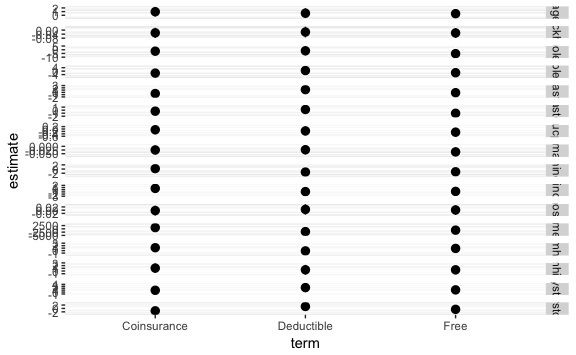
\includegraphics[width=0.7\linewidth]{rand_files/figure-latex/unnamed-chunk-6-1} \end{center}

\hypertarget{table-1.4}{%
\section{Table 1.4}\label{table-1.4}}

Replicate Angrist and Pischke (2014) Table 1.4 which presents health
outcome and health expenditure results from the RAND HIE.

\begin{Shaded}
\begin{Highlighting}[]
\KeywordTok{data}\NormalTok{(}\StringTok{"rand_person_spend"}\NormalTok{, }\DataTypeTok{package =} \StringTok{"masteringmetrics"}\NormalTok{)}
\end{Highlighting}
\end{Shaded}

Correlate year variable from annual expenditures data to correct
calendar year in order to adjust for inflation.

\begin{Shaded}
\begin{Highlighting}[]
\NormalTok{rand_person_spend <-}\StringTok{ }\KeywordTok{mutate}\NormalTok{(rand_person_spend,}
                            \DataTypeTok{expyear =}\NormalTok{ indv_start_year }\OperatorTok{+}\StringTok{ }\NormalTok{year }\OperatorTok{-}\StringTok{ }\DecValTok{1}\NormalTok{)}
\end{Highlighting}
\end{Shaded}

Adjust spending for inflation. The CPI adjustment values below are based
on the June CPI from 1991 (see table found at
\url{http://www.seattle.gov/financedepartment/cpi/historical.htm}).

\begin{Shaded}
\begin{Highlighting}[]
\NormalTok{cpi <-}\StringTok{ }\KeywordTok{tribble}\NormalTok{(}
  \OperatorTok{~}\StringTok{ }\NormalTok{year, }\OperatorTok{~}\StringTok{ }\NormalTok{cpi,}
  \DecValTok{1973}\NormalTok{, }\FloatTok{3.07}\NormalTok{,}
  \DecValTok{1974}\NormalTok{, }\FloatTok{2.76}\NormalTok{,}
  \DecValTok{1975}\NormalTok{, }\FloatTok{2.53}\NormalTok{,}
  \DecValTok{1976}\NormalTok{, }\FloatTok{2.39}\NormalTok{,}
  \DecValTok{1977}\NormalTok{, }\FloatTok{2.24}\NormalTok{,}
  \DecValTok{1978}\NormalTok{, }\FloatTok{2.09}\NormalTok{,}
  \DecValTok{1979}\NormalTok{, }\FloatTok{1.88}\NormalTok{,}
  \DecValTok{1980}\NormalTok{, }\FloatTok{1.65}\NormalTok{,}
  \DecValTok{1981}\NormalTok{, }\FloatTok{1.5}\NormalTok{,}
  \DecValTok{1982}\NormalTok{, }\FloatTok{1.41}\NormalTok{,}
  \DecValTok{1983}\NormalTok{, }\FloatTok{1.37}\NormalTok{,}
  \DecValTok{1984}\NormalTok{, }\FloatTok{1.31}\NormalTok{,}
  \DecValTok{1985}\NormalTok{, }\FloatTok{1.27}
\NormalTok{)}
\end{Highlighting}
\end{Shaded}

\begin{Shaded}
\begin{Highlighting}[]
\NormalTok{rand_person_spend <-}\StringTok{ }\KeywordTok{left_join}\NormalTok{(rand_person_spend,}
\NormalTok{                               cpi, }\DataTypeTok{by =} \KeywordTok{c}\NormalTok{(}\StringTok{"expyear"}\NormalTok{ =}\StringTok{ "year"}\NormalTok{)) }\OperatorTok
\StringTok{  }\KeywordTok{mutate}\NormalTok{(}\DataTypeTok{out_inf =}\NormalTok{ outsum }\OperatorTok{*}\StringTok{ }\NormalTok{cpi,}
         \DataTypeTok{inpdol_inf =}\NormalTok{ inpdol }\OperatorTok{*}\StringTok{ }\NormalTok{cpi)}
\end{Highlighting}
\end{Shaded}

Add a total spending variable.

\begin{Shaded}
\begin{Highlighting}[]
\NormalTok{rand_person_spend <-}\StringTok{ }\KeywordTok{mutate}\NormalTok{(rand_person_spend,}
                       \DataTypeTok{tot_inf =}\NormalTok{ inpdol_inf }\OperatorTok{+}\StringTok{ }\NormalTok{out_inf)}
\end{Highlighting}
\end{Shaded}

Add a variable for any health insurance (free, Individual deductible, or
cost-sharing):

\begin{Shaded}
\begin{Highlighting}[]
\NormalTok{rand_person_spend <-}\StringTok{ }\KeywordTok{mutate}\NormalTok{(rand_person_spend,}
                            \DataTypeTok{any_ins =}\NormalTok{ plantype }\OperatorTok{!=}\StringTok{ "Catastrophic"}\NormalTok{)}
\end{Highlighting}
\end{Shaded}

Count the number of observations in each plan-type,

\begin{Shaded}
\begin{Highlighting}[]
\KeywordTok{count}\NormalTok{(rand_person_spend, plantype)}
\CommentTok{#> # A tibble: 4 x 2}
\CommentTok{#>   plantype         n}
\CommentTok{#>   <fct>        <int>}
\CommentTok{#> 1 Catastrophic  3724}
\CommentTok{#> 2 Deductible    4175}
\CommentTok{#> 3 Cost Sharing  5464}
\CommentTok{#> 4 Free          6840}
\end{Highlighting}
\end{Shaded}

and any-insurance,

\begin{Shaded}
\begin{Highlighting}[]
\KeywordTok{count}\NormalTok{(rand_person_spend, any_ins)}
\CommentTok{#> # A tibble: 2 x 2}
\CommentTok{#>   any_ins     n}
\CommentTok{#>   <lgl>   <int>}
\CommentTok{#> 1 FALSE    3724}
\CommentTok{#> 2 TRUE    16479}
\end{Highlighting}
\end{Shaded}

Create a list of response variables.

\begin{Shaded}
\begin{Highlighting}[]
\NormalTok{varlist <-}\StringTok{ }\KeywordTok{c}\NormalTok{(}\StringTok{"ftf"}\NormalTok{, }\StringTok{"out_inf"}\NormalTok{, }\StringTok{"totadm"}\NormalTok{, }\StringTok{"inpdol_inf"}\NormalTok{, }\StringTok{"tot_inf"}\NormalTok{)}
\end{Highlighting}
\end{Shaded}

Calculate the mean and standard deviation for those receiving
catastrophic insurance.

\begin{Shaded}
\begin{Highlighting}[]
\NormalTok{rand_person_spend }\OperatorTok
\StringTok{  }\KeywordTok{filter}\NormalTok{(plantype }\OperatorTok{==}\StringTok{ "Catastrophic"}\NormalTok{) }\OperatorTok
\StringTok{  }\KeywordTok{select}\NormalTok{(}\KeywordTok{one_of}\NormalTok{(varlist)) }\OperatorTok
\StringTok{  }\KeywordTok{gather}\NormalTok{(response, value) }\OperatorTok
\StringTok{  }\KeywordTok{group_by}\NormalTok{(response) }\OperatorTok
\StringTok{  }\KeywordTok{summarise}\NormalTok{(}\DataTypeTok{Mean =} \KeywordTok{mean}\NormalTok{(value, }\DataTypeTok{na.rm =} \OtherTok{TRUE}\NormalTok{),}
            \StringTok{`}\DataTypeTok{Std. Dev.}\StringTok{`}\NormalTok{ =}\StringTok{ }\KeywordTok{sd}\NormalTok{(value, }\DataTypeTok{na.rm =} \OtherTok{TRUE}\NormalTok{))}
\CommentTok{#> # A tibble: 5 x 3}
\CommentTok{#>   response       Mean `Std. Dev.`}
\CommentTok{#>   <chr>         <dbl>       <dbl>}
\CommentTok{#> 1 ftf          2.78         5.50 }
\CommentTok{#> 2 inpdol_inf 388.        2308.   }
\CommentTok{#> 3 out_inf    248.         488.   }
\CommentTok{#> 4 tot_inf    636.        2535.   }
\CommentTok{#> 5 totadm       0.0991       0.379}
\end{Highlighting}
\end{Shaded}

Calculate the difference in means between plans and the catastophic
plan.

\begin{Shaded}
\begin{Highlighting}[]
\NormalTok{calc_diffs <-}\StringTok{ }\ControlFlowTok{function}\NormalTok{(x) \{}
  \CommentTok{# programmatically create the formula}
\NormalTok{  f <-}\StringTok{ }\KeywordTok{quo}\NormalTok{(}\OperatorTok{!!}\KeywordTok{sym}\NormalTok{(x) }\OperatorTok{~}\StringTok{ }\NormalTok{plantype)}

\NormalTok{  mod <-}\StringTok{ }\KeywordTok{lm}\NormalTok{(f, }\DataTypeTok{data =}\NormalTok{ rand_person_spend)  }\CommentTok{# nolint}
\NormalTok{  out <-}\StringTok{ }\KeywordTok{cluster_se}\NormalTok{(mod, }\DataTypeTok{cluster =}\NormalTok{ rand_person_spend[[}\StringTok{"fam_identifier"}\NormalTok{]])}
\NormalTok{  out[[}\StringTok{"response"}\NormalTok{]] <-}\StringTok{ }\NormalTok{x}
\NormalTok{  out}
\NormalTok{\}}
\end{Highlighting}
\end{Shaded}

\begin{Shaded}
\begin{Highlighting}[]
\NormalTok{person_diffs <-}\StringTok{ }\KeywordTok{map_dfr}\NormalTok{(varlist, calc_diffs) }\OperatorTok
\StringTok{  }\KeywordTok{select}\NormalTok{(response, term, estimate, std.error) }\OperatorTok
\StringTok{  }\KeywordTok{mutate}\NormalTok{(}\DataTypeTok{term =} \KeywordTok{str_replace}\NormalTok{(term, }\StringTok{"^plantype"}\NormalTok{, }\StringTok{""}\NormalTok{))}
\end{Highlighting}
\end{Shaded}

Standard errors are clustered by family identifier using the
\textbf{clubSandwich} package.

Print the table. If this were an actual publication, I'd make it nicer.

\begin{Shaded}
\begin{Highlighting}[]
\NormalTok{fmt_num <-}\StringTok{ }\ControlFlowTok{function}\NormalTok{(x) \{}
  \KeywordTok{prettyNum}\NormalTok{(x, }\DataTypeTok{digits =} \DecValTok{3}\NormalTok{, }\DataTypeTok{format =} \StringTok{"f"}\NormalTok{, }\DataTypeTok{big.mark =} \StringTok{","}\NormalTok{, }\DataTypeTok{drop0trailing =} \OtherTok{FALSE}\NormalTok{)}
\NormalTok{\}}

\NormalTok{person_diffs }\OperatorTok
\StringTok{  }\KeywordTok{mutate}\NormalTok{(}\DataTypeTok{estimate =} \KeywordTok{str_c}\NormalTok{(}\KeywordTok{fmt_num}\NormalTok{(estimate), }\StringTok{" ("}\NormalTok{, }\KeywordTok{fmt_num}\NormalTok{(std.error), }\StringTok{")"}\NormalTok{)) }\OperatorTok
\StringTok{  }\KeywordTok{select}\NormalTok{(}\OperatorTok{-}\NormalTok{std.error) }\OperatorTok
\StringTok{  }\KeywordTok{spread}\NormalTok{(term, estimate) }\OperatorTok
\StringTok{  }\NormalTok{knitr}\OperatorTok{::}\KeywordTok{kable}\NormalTok{(}\DataTypeTok{digits =} \DecValTok{3}\NormalTok{)}
\end{Highlighting}
\end{Shaded}

\begin{tabular}{l|l|l|l|l}
\hline
response & (Intercept) & Cost Sharing & Deductible & Free\\
\hline
ftf & 2.78 (0.178) & 0.481 (0.24) & 0.193 (0.247) & 1.66 (0.248)\\
\hline
inpdol\_inf & 388 (44.9) & 92.5 (72.8) & 72.2 (68.6) & 116 (59.8)\\
\hline
out\_inf & 248 (14.8) & 59.8 (20.7) & 41.8 (20.8) & 169 (19.9)\\
\hline
tot\_inf & 636 (54.5) & 152 (84.6) & 114 (79.1) & 285 (72.4)\\
\hline
totadm & 0.0991 (0.00785) & 0.0023 (0.0108) & 0.0159 (0.0109) & 0.0288 (0.0105)\\
\hline
\end{tabular}

Additionally we could plot the difference-in-means of each plan type
vs.~catastrophic insurance.

\begin{Shaded}
\begin{Highlighting}[]
\KeywordTok{ggplot}\NormalTok{(}\KeywordTok{filter}\NormalTok{(person_diffs, term }\OperatorTok{!=}\StringTok{ "(Intercept)"}\NormalTok{),}
              \KeywordTok{aes}\NormalTok{(}\DataTypeTok{x =}\NormalTok{ term, }\DataTypeTok{y =}\NormalTok{ estimate,}
                  \DataTypeTok{ymin =}\NormalTok{ estimate }\OperatorTok{-}\StringTok{ }\DecValTok{2} \OperatorTok{*}\StringTok{ }\NormalTok{std.error,}
                  \DataTypeTok{ymax =}\NormalTok{ estimate }\OperatorTok{+}\StringTok{ }\DecValTok{2} \OperatorTok{*}\StringTok{ }\NormalTok{std.error)) }\OperatorTok{+}
\StringTok{  }\KeywordTok{geom_hline}\NormalTok{(}\DataTypeTok{yintercept =} \DecValTok{0}\NormalTok{, }\DataTypeTok{colour =} \StringTok{"white"}\NormalTok{, }\DataTypeTok{size =} \DecValTok{1}\NormalTok{) }\OperatorTok{+}
\StringTok{  }\KeywordTok{geom_pointrange}\NormalTok{() }\OperatorTok{+}
\StringTok{  }\KeywordTok{facet_grid}\NormalTok{(response }\OperatorTok{~}\StringTok{ }\NormalTok{., }\DataTypeTok{scales =} \StringTok{"free_y"}\NormalTok{)}
\end{Highlighting}
\end{Shaded}

\begin{center}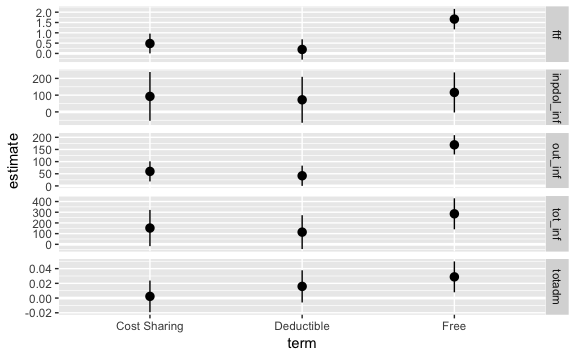
\includegraphics[width=0.7\linewidth]{rand_files/figure-latex/unnamed-chunk-14-1} \end{center}

\hypertarget{references-1}{%
\section*{References}\label{references-1}}
\addcontentsline{toc}{section}{References}

\begin{itemize}
\tightlist
\item
  \url{https://www.icpsr.umich.edu/icpsrweb/NACDA/studies/6439/version/1}
\item
  \url{http://masteringmetrics.com/wp-content/uploads/2015/01/ReadMe_RAND.txt}
\item
  \url{http://masteringmetrics.com/wp-content/uploads/2015/01/Code.zip}
\end{itemize}

\hypertarget{part-chapter-3}{%
\part{Chapter 3}\label{part-chapter-3}}

\hypertarget{minneapolis-domestic-violence-experiment}{%
\chapter{Minneapolis Domestic Violence
Experiment}\label{minneapolis-domestic-violence-experiment}}

This replicates Table 3.3 of \emph{Mastering 'Metrics}, which replicates
the Minneapolis Domestic Violence Experiment (Sherman and Berk
1984,@Angrist2006).

Load necessary packages.

\begin{Shaded}
\begin{Highlighting}[]
\KeywordTok{library}\NormalTok{(}\StringTok{"tidyverse"}\NormalTok{)}
\end{Highlighting}
\end{Shaded}

Load the MDVE data.

\begin{Shaded}
\begin{Highlighting}[]
\KeywordTok{data}\NormalTok{(}\StringTok{"mdve"}\NormalTok{, }\DataTypeTok{package =} \StringTok{"masteringmetrics"}\NormalTok{)}
\end{Highlighting}
\end{Shaded}

Randomized assignments (i.e.~what are police assigned to do) are in the
\texttt{assigned} column. Actual outcomes (i.e.~what action do the
police actually take) is in the \texttt{outcome} column. gen outcome =
``Arrest'' if T\_FINAL == 1 replace outcome = ``Advise'' if T\_FINAL ==
2 replace outcome = ``Separate'' if T\_FINAL == 3 replace outcome =
``Other'' if T\_FINAL == 4 gen total = 1

\begin{Shaded}
\begin{Highlighting}[]
\NormalTok{mdve <-}\StringTok{ }\KeywordTok{mutate}\NormalTok{(mdve,}
               \DataTypeTok{assigned =} \KeywordTok{case_when}\NormalTok{(}
\NormalTok{      T_RANDOM }\OperatorTok{==}\StringTok{ }\DecValTok{1} \OperatorTok{~}\StringTok{ "Arrest"}\NormalTok{,}
\NormalTok{      T_RANDOM }\OperatorTok{==}\StringTok{ }\DecValTok{2} \OperatorTok{~}\StringTok{ "Advise"}\NormalTok{,}
\NormalTok{      T_RANDOM }\OperatorTok{==}\StringTok{ }\DecValTok{3} \OperatorTok{~}\StringTok{ "Separate"}
\NormalTok{    ),}
      \DataTypeTok{outcome =} \KeywordTok{case_when}\NormalTok{(}
\NormalTok{        T_FINAL }\OperatorTok{==}\StringTok{ }\DecValTok{1} \OperatorTok{~}\StringTok{ "Arrest"}\NormalTok{,}
\NormalTok{        T_FINAL }\OperatorTok{==}\StringTok{ }\DecValTok{2} \OperatorTok{~}\StringTok{ "Advise"}\NormalTok{,}
\NormalTok{        T_FINAL }\OperatorTok{==}\StringTok{ }\DecValTok{3} \OperatorTok{~}\StringTok{ "Separate"}\NormalTok{,}
\NormalTok{        T_FINAL }\OperatorTok{==}\StringTok{ }\DecValTok{4} \OperatorTok{~}\StringTok{ "Other"}
\NormalTok{      ),}
      \DataTypeTok{coddled_a =}\NormalTok{ assigned }\OperatorTok{!=}\StringTok{ "Arrest"}\NormalTok{,}
      \DataTypeTok{coddled_o =}\NormalTok{ outcome }\OperatorTok{!=}\StringTok{ "Arrest"}
\NormalTok{    ) }\OperatorTok
\StringTok{  }\KeywordTok{filter}\NormalTok{(outcome }\OperatorTok{!=}\StringTok{ "Other"}\NormalTok{)}
\end{Highlighting}
\end{Shaded}

Assigned and delivered treatments in the MDVE:

\begin{Shaded}
\begin{Highlighting}[]
\NormalTok{mdve_summary <-}
\StringTok{  }\NormalTok{mdve }\OperatorTok
\StringTok{  }\KeywordTok{count}\NormalTok{(assigned, outcome) }\OperatorTok
\StringTok{  }\KeywordTok{group_by}\NormalTok{(assigned) }\OperatorTok
\StringTok{  }\KeywordTok{mutate}\NormalTok{(}\DataTypeTok{p =}\NormalTok{ n }\OperatorTok{/}\StringTok{ }\KeywordTok{sum}\NormalTok{(n))}
\KeywordTok{print}\NormalTok{(mdve_summary, }\DataTypeTok{n =} \KeywordTok{nrow}\NormalTok{(mdve_summary))}
\CommentTok{#> # A tibble: 8 x 4}
\CommentTok{#> # Groups:   assigned [3]}
\CommentTok{#>   assigned outcome      n      p}
\CommentTok{#>   <chr>    <chr>    <int>  <dbl>}
\CommentTok{#> 1 Advise   Advise      84 0.778 }
\CommentTok{#> 2 Advise   Arrest      19 0.176 }
\CommentTok{#> 3 Advise   Separate     5 0.0463}
\CommentTok{#> 4 Arrest   Arrest      91 0.989 }
\CommentTok{#> 5 Arrest   Separate     1 0.0109}
\CommentTok{#> 6 Separate Advise       5 0.0439}
\CommentTok{#> 7 Separate Arrest      26 0.228 }
\CommentTok{#> 8 Separate Separate    83 0.728}
\end{Highlighting}
\end{Shaded}

Assigned proportions in the MDVE:

\begin{Shaded}
\begin{Highlighting}[]
\NormalTok{mdve_assigned <-}\StringTok{ }\NormalTok{mdve }\OperatorTok
\StringTok{  }\KeywordTok{count}\NormalTok{(assigned) }\OperatorTok
\StringTok{  }\KeywordTok{mutate}\NormalTok{(}\DataTypeTok{p =}\NormalTok{ n }\OperatorTok{/}\StringTok{ }\KeywordTok{sum}\NormalTok{(n))}
\NormalTok{mdve_assigned}
\CommentTok{#> # A tibble: 3 x 3}
\CommentTok{#>   assigned     n     p}
\CommentTok{#>   <chr>    <int> <dbl>}
\CommentTok{#> 1 Advise     108 0.344}
\CommentTok{#> 2 Arrest      92 0.293}
\CommentTok{#> 3 Separate   114 0.363}
\end{Highlighting}
\end{Shaded}

Delivered treatments in the MDVE:

\begin{Shaded}
\begin{Highlighting}[]
\NormalTok{mdve_outcome <-}\StringTok{ }\NormalTok{mdve }\OperatorTok
\StringTok{  }\KeywordTok{count}\NormalTok{(outcome) }\OperatorTok
\StringTok{  }\KeywordTok{mutate}\NormalTok{(}\DataTypeTok{p =}\NormalTok{ n }\OperatorTok{/}\StringTok{ }\KeywordTok{sum}\NormalTok{(n))}
\NormalTok{mdve_outcome}
\CommentTok{#> # A tibble: 3 x 3}
\CommentTok{#>   outcome      n     p}
\CommentTok{#>   <chr>    <int> <dbl>}
\CommentTok{#> 1 Advise      89 0.283}
\CommentTok{#> 2 Arrest     136 0.433}
\CommentTok{#> 3 Separate    89 0.283}
\end{Highlighting}
\end{Shaded}

Probability of being coddled, given being assigned the coddled
treatment:

\begin{Shaded}
\begin{Highlighting}[]
\NormalTok{mdve_coddled <-}\StringTok{ }\NormalTok{mdve }\OperatorTok
\StringTok{  }\KeywordTok{count}\NormalTok{(coddled_a, coddled_o) }\OperatorTok
\StringTok{  }\KeywordTok{group_by}\NormalTok{(coddled_a) }\OperatorTok
\StringTok{  }\KeywordTok{mutate}\NormalTok{(}\DataTypeTok{p =}\NormalTok{ n }\OperatorTok{/}\StringTok{ }\KeywordTok{sum}\NormalTok{(n))}
\NormalTok{mdve_coddled}
\CommentTok{#> # A tibble: 4 x 4}
\CommentTok{#> # Groups:   coddled_a [2]}
\CommentTok{#>   coddled_a coddled_o     n      p}
\CommentTok{#>   <lgl>     <lgl>     <int>  <dbl>}
\CommentTok{#> 1 FALSE     FALSE        91 0.989 }
\CommentTok{#> 2 FALSE     TRUE          1 0.0109}
\CommentTok{#> 3 TRUE      FALSE        45 0.203 }
\CommentTok{#> 4 TRUE      TRUE        177 0.797}
\end{Highlighting}
\end{Shaded}

IV first stage, \[
E[D_i | Z_i = 1] - E[D_i | Z_i = 0] .
\]

\begin{Shaded}
\begin{Highlighting}[]
\KeywordTok{filter}\NormalTok{(mdve_coddled, coddled_o, coddled_a)}\OperatorTok{$}\NormalTok{p }\OperatorTok{-}
\StringTok{  }\KeywordTok{filter}\NormalTok{(mdve_coddled, coddled_o, }\OperatorTok{!}\NormalTok{coddled_a)}\OperatorTok{$}\NormalTok{p}
\CommentTok{#> [1] 0.786}
\end{Highlighting}
\end{Shaded}

The response variable is not provided, so the full 2SLS is not estimated
here.

\hypertarget{references-2}{%
\section{References}\label{references-2}}

\begin{itemize}
\tightlist
\item
  \url{http://masteringmetrics.com/wp-content/uploads/2015/02/MDVE_Table33.do}
\item
  \url{http://masteringmetrics.com/wp-content/uploads/2015/02/ReadMe_MDVE.txt}
\end{itemize}

\hypertarget{part-chapter-4}{%
\part{Chapter 4}\label{part-chapter-4}}

\hypertarget{mlda-regression-discontinuity}{%
\chapter{MLDA Regression
Discontinuity}\label{mlda-regression-discontinuity}}

MLDA Regression Discontinuity (based on data from Carpenter and Dobkin
(2011)) from Chapter 4 of \emph{Mastering 'Metrics}, Table 4.1 and
Figures 4.2, 4.4, and 4.5 in Mastering Metrics. These present sharp RD
estimates of the effect of the minimum legal drinking age (MLDA) on
mortality.

Load libraries.

\begin{Shaded}
\begin{Highlighting}[]
\KeywordTok{library}\NormalTok{(}\StringTok{"tidyverse"}\NormalTok{)}
\KeywordTok{library}\NormalTok{(}\StringTok{"haven"}\NormalTok{)}
\KeywordTok{library}\NormalTok{(}\StringTok{"rlang"}\NormalTok{)}
\KeywordTok{library}\NormalTok{(}\StringTok{"broom"}\NormalTok{)}
\KeywordTok{library}\NormalTok{(}\StringTok{"lmtest"}\NormalTok{)}
\KeywordTok{library}\NormalTok{(}\StringTok{"sandwich"}\NormalTok{)}
\end{Highlighting}
\end{Shaded}

Load MLDA data

\begin{Shaded}
\begin{Highlighting}[]
\KeywordTok{data}\NormalTok{(}\StringTok{"mlda"}\NormalTok{, }\DataTypeTok{package =} \StringTok{"masteringmetrics"}\NormalTok{)}
\end{Highlighting}
\end{Shaded}

Add an indicator variable for individuals over 21 years of age.

\begin{Shaded}
\begin{Highlighting}[]
\NormalTok{mlda <-}\StringTok{ }\KeywordTok{mutate}\NormalTok{(mlda,}
               \DataTypeTok{age =}\NormalTok{ agecell }\OperatorTok{-}\StringTok{ }\DecValTok{21}\NormalTok{,}
               \DataTypeTok{over21 =} \KeywordTok{as.integer}\NormalTok{(agecell }\OperatorTok{>=}\StringTok{ }\DecValTok{21}\NormalTok{))}
\end{Highlighting}
\end{Shaded}

Add a variable for other causes of death.

\begin{Shaded}
\begin{Highlighting}[]
\NormalTok{mlda <-}\StringTok{ }\KeywordTok{mutate}\NormalTok{(mlda, }\DataTypeTok{ext_oth =}\NormalTok{ external }\OperatorTok{-}\StringTok{ }\NormalTok{homicide }\OperatorTok{-}\StringTok{ }\NormalTok{suicide }\OperatorTok{-}\StringTok{ }\NormalTok{mva)}
\end{Highlighting}
\end{Shaded}

For ``all causes'', ``motor vehicle accidents'', and ``internal causes''
deaths plot the linear and quadratic trends on each side of age 21.

\begin{Shaded}
\begin{Highlighting}[]
\NormalTok{varlist <-}\StringTok{ }\KeywordTok{c}\NormalTok{(}\StringTok{"all"}\NormalTok{ =}\StringTok{ "All Causes"}\NormalTok{,}
             \StringTok{"mva"}\NormalTok{ =}\StringTok{ "Motor Vehicle Accidents"}\NormalTok{,}
             \StringTok{"internal"}\NormalTok{ =}\StringTok{ "Internal Causes"}\NormalTok{)}
\end{Highlighting}
\end{Shaded}

\begin{Shaded}
\begin{Highlighting}[]
\NormalTok{mlda }\OperatorTok
\StringTok{  }\KeywordTok{select}\NormalTok{(agecell, over21, }\KeywordTok{one_of}\NormalTok{(}\KeywordTok{names}\NormalTok{(varlist))) }\OperatorTok
\StringTok{  }\KeywordTok{gather}\NormalTok{(response, value, }\OperatorTok{-}\NormalTok{agecell, }\OperatorTok{-}\NormalTok{over21, }\DataTypeTok{na.rm =} \OtherTok{TRUE}\NormalTok{) }\OperatorTok
\StringTok{  }\KeywordTok{mutate}\NormalTok{(}\DataTypeTok{response =} \KeywordTok{recode}\NormalTok{(response, }\OperatorTok{!!!}\KeywordTok{as.list}\NormalTok{(varlist))) }\OperatorTok
\StringTok{  }\KeywordTok{ggplot}\NormalTok{(}\KeywordTok{aes}\NormalTok{(}\DataTypeTok{x =}\NormalTok{ agecell, }\DataTypeTok{y =}\NormalTok{ value)) }\OperatorTok{+}
\StringTok{  }\KeywordTok{geom_point}\NormalTok{() }\OperatorTok{+}
\StringTok{  }\KeywordTok{geom_smooth}\NormalTok{(}\DataTypeTok{mapping =} \KeywordTok{aes}\NormalTok{(}\DataTypeTok{group =}\NormalTok{ over21), }\DataTypeTok{se =} \OtherTok{FALSE}\NormalTok{, }\DataTypeTok{method =} \StringTok{"lm"}\NormalTok{,}
              \DataTypeTok{formula =}\NormalTok{ y }\OperatorTok{~}\StringTok{ }\KeywordTok{poly}\NormalTok{(x, }\DecValTok{2}\NormalTok{)) }\OperatorTok{+}
\StringTok{  }\KeywordTok{geom_smooth}\NormalTok{(}\DataTypeTok{mapping =} \KeywordTok{aes}\NormalTok{(}\DataTypeTok{group =}\NormalTok{ over21), }\DataTypeTok{se =} \OtherTok{FALSE}\NormalTok{, }\DataTypeTok{method =} \StringTok{"lm"}\NormalTok{,}
              \DataTypeTok{formula =}\NormalTok{ y }\OperatorTok{~}\StringTok{ }\NormalTok{x, }\DataTypeTok{color =} \StringTok{"black"}\NormalTok{) }\OperatorTok{+}
\StringTok{  }\KeywordTok{facet_grid}\NormalTok{(response }\OperatorTok{~}\StringTok{ }\NormalTok{., }\DataTypeTok{scales =} \StringTok{"free_y"}\NormalTok{) }\OperatorTok{+}
\StringTok{  }\KeywordTok{labs}\NormalTok{(}\DataTypeTok{y =} \StringTok{"Mortality rate (per 100,000)"}\NormalTok{, }\DataTypeTok{x =} \StringTok{"Age"}\NormalTok{)}
\end{Highlighting}
\end{Shaded}

\begin{center}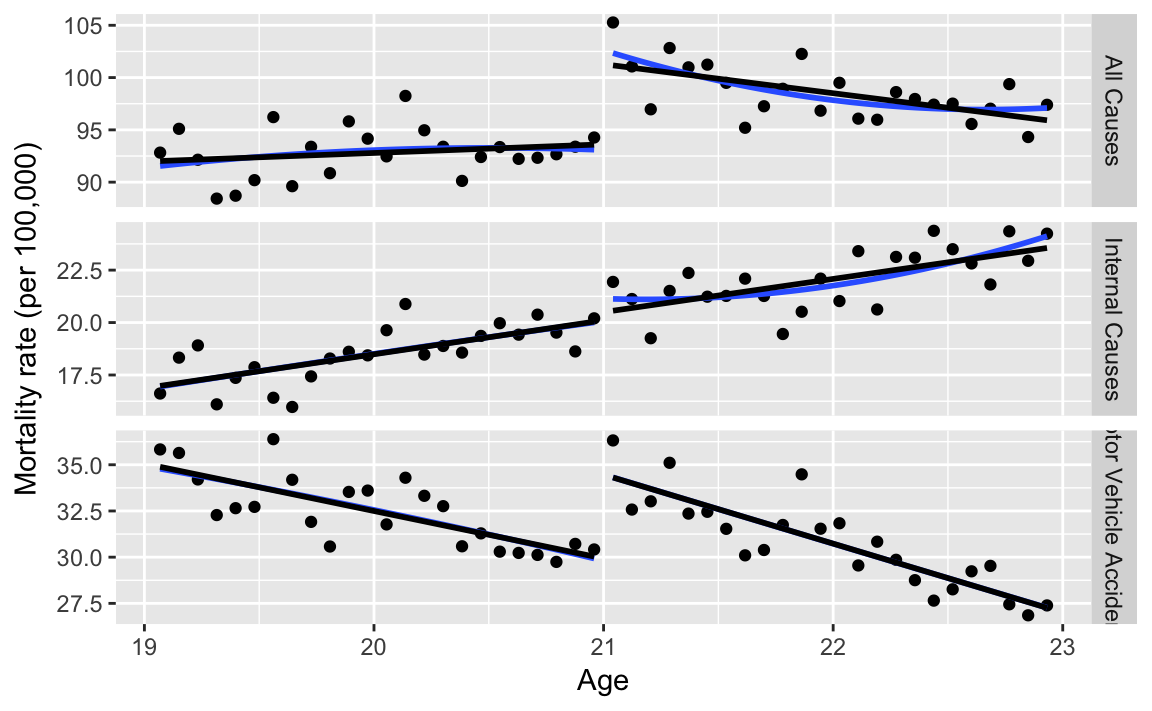
\includegraphics[width=0.7\linewidth]{mlda-rd_files/figure-latex/unnamed-chunk-4-1} \end{center}

\begin{Shaded}
\begin{Highlighting}[]
\NormalTok{responses <-}\StringTok{ }\KeywordTok{c}\NormalTok{(}\StringTok{"all"}\NormalTok{ =}\StringTok{ "All deaths"}\NormalTok{,}
               \StringTok{"mva"}\NormalTok{ =}\StringTok{ "Motor vehicle accidents"}\NormalTok{,}
               \StringTok{"suicide"}\NormalTok{ =}\StringTok{ "Suicide"}\NormalTok{,}
               \StringTok{"homicide"}\NormalTok{ =}\StringTok{ "Homocide"}\NormalTok{,}
               \StringTok{"ext_oth"}\NormalTok{ =}\StringTok{ "Other external causes"}\NormalTok{,}
               \StringTok{"internal"}\NormalTok{ =}\StringTok{ "All internal causes"}\NormalTok{,}
               \StringTok{"alcohol"}\NormalTok{ =}\StringTok{ "Alcohol"}\NormalTok{)}
\end{Highlighting}
\end{Shaded}

Define a function to run four regressions for a given response variable,
\texttt{y}.

\begin{Shaded}
\begin{Highlighting}[]
\NormalTok{run_reg <-}\StringTok{ }\ControlFlowTok{function}\NormalTok{(y) \{}
\NormalTok{  mods <-}\StringTok{ }\KeywordTok{list}\NormalTok{(}
    \StringTok{"Ages 19-22, Linear"}\NormalTok{ =}
\StringTok{      }\KeywordTok{lm}\NormalTok{(}\KeywordTok{quo}\NormalTok{(}\OperatorTok{!!}\KeywordTok{sym}\NormalTok{(y) }\OperatorTok{~}\StringTok{ }\NormalTok{age }\OperatorTok{*}\StringTok{ }\NormalTok{over21), }\DataTypeTok{data =}\NormalTok{ mlda),}
    \StringTok{"Ages 19-22, Quadratic"}\NormalTok{ =}
\StringTok{      }\KeywordTok{lm}\NormalTok{(}\KeywordTok{quo}\NormalTok{(}\OperatorTok{!!}\KeywordTok{sym}\NormalTok{(y) }\OperatorTok{~}\StringTok{ }\KeywordTok{poly}\NormalTok{(age, }\DecValTok{2}\NormalTok{, }\DataTypeTok{raw =} \OtherTok{TRUE}\NormalTok{) }\OperatorTok{*}\StringTok{ }\NormalTok{over21), }\DataTypeTok{data =}\NormalTok{ mlda),}
    \StringTok{"Ages 20-21, Linear"}\NormalTok{ =}
\StringTok{      }\KeywordTok{lm}\NormalTok{(}\KeywordTok{quo}\NormalTok{(}\OperatorTok{!!}\KeywordTok{sym}\NormalTok{(y) }\OperatorTok{~}\StringTok{ }\NormalTok{age }\OperatorTok{*}\StringTok{ }\NormalTok{over21),}
             \DataTypeTok{data =} \KeywordTok{filter}\NormalTok{(mlda, agecell }\OperatorTok{>=}\StringTok{ }\DecValTok{20}\NormalTok{, agecell }\OperatorTok{<=}\StringTok{ }\DecValTok{22}\NormalTok{)),}
    \StringTok{"Ages 20-21, Quadratic"}\NormalTok{ =}
\StringTok{      }\KeywordTok{lm}\NormalTok{(}\KeywordTok{quo}\NormalTok{(}\OperatorTok{!!}\KeywordTok{sym}\NormalTok{(y) }\OperatorTok{~}\StringTok{ }\KeywordTok{poly}\NormalTok{(age, }\DecValTok{2}\NormalTok{, }\DataTypeTok{raw =} \OtherTok{TRUE}\NormalTok{) }\OperatorTok{*}\StringTok{ }\NormalTok{over21),}
             \DataTypeTok{data =} \KeywordTok{filter}\NormalTok{(mlda, agecell }\OperatorTok{>=}\StringTok{ }\DecValTok{20}\NormalTok{, agecell }\OperatorTok{<=}\StringTok{ }\DecValTok{22}\NormalTok{))}
\NormalTok{  )}
\NormalTok{  out <-}\StringTok{ }\KeywordTok{tibble}\NormalTok{(}
    \DataTypeTok{model_name =} \KeywordTok{names}\NormalTok{(mods),}
    \DataTypeTok{model =}\NormalTok{ mods,}
    \DataTypeTok{ages =} \KeywordTok{rep}\NormalTok{(}\KeywordTok{c}\NormalTok{(}\StringTok{"19-22"}\NormalTok{, }\StringTok{"20-21"}\NormalTok{), }\DataTypeTok{each =} \DecValTok{2}\NormalTok{),}
    \DataTypeTok{trend =} \KeywordTok{rep}\NormalTok{(}\KeywordTok{c}\NormalTok{(}\StringTok{"Linear"}\NormalTok{, }\StringTok{"Quadratic"}\NormalTok{), }\DecValTok{2}\NormalTok{),}
    \DataTypeTok{model_num =} \KeywordTok{seq_along}\NormalTok{(mods)}
\NormalTok{  ) }\OperatorTok
\StringTok{    }\KeywordTok{mutate}\NormalTok{(}\DataTypeTok{coefs =} \KeywordTok{map}\NormalTok{(model, }\OperatorTok{~}\StringTok{ }\KeywordTok{tidy}\NormalTok{(}\KeywordTok{coeftest}\NormalTok{(.x, }\KeywordTok{vcovHC}\NormalTok{(.x))))) }\OperatorTok\StringTok{ }\CommentTok{# nolint}
\StringTok{    }\KeywordTok{unnest}\NormalTok{(coefs, }\DataTypeTok{.drop =} \OtherTok{FALSE}\NormalTok{) }\OperatorTok
\StringTok{    }\KeywordTok{filter}\NormalTok{(term }\OperatorTok{==}\StringTok{ "over21"}\NormalTok{) }\OperatorTok
\StringTok{    }\KeywordTok{select}\NormalTok{(model_name, model, term, estimate, std.error) }\OperatorTok
\StringTok{    }\KeywordTok{mutate}\NormalTok{(}\DataTypeTok{response =}\NormalTok{ y)}
  \CommentTok{# sample size = df.residuals + residuals}
\NormalTok{  out[[}\StringTok{"obs"}\NormalTok{]] <-}\StringTok{ }\KeywordTok{map_dfr}\NormalTok{(mods, glance) }\OperatorTok
\StringTok{    }\KeywordTok{mutate}\NormalTok{(}\DataTypeTok{obs =}\NormalTok{ df.residual }\OperatorTok{+}\StringTok{ }\NormalTok{df) }\OperatorTok
\StringTok{    }\KeywordTok{pluck}\NormalTok{(}\StringTok{"obs"}\NormalTok{)}
\NormalTok{  out}
\NormalTok{\}}

\NormalTok{mlda_regs <-}\StringTok{ }\KeywordTok{map_dfr}\NormalTok{(}\KeywordTok{names}\NormalTok{(responses), run_reg) }\OperatorTok
\StringTok{  }\KeywordTok{mutate}\NormalTok{(}\DataTypeTok{response =} \KeywordTok{recode}\NormalTok{(response, }\OperatorTok{!!!}\KeywordTok{as.list}\NormalTok{(responses)))}
\end{Highlighting}
\end{Shaded}

\begin{Shaded}
\begin{Highlighting}[]
\NormalTok{mlda_regs }\OperatorTok
\StringTok{  }\KeywordTok{select}\NormalTok{(model_name, response, estimate, std.error) }\OperatorTok
\StringTok{  }\KeywordTok{gather}\NormalTok{(stat, value, estimate, std.error) }\OperatorTok
\StringTok{  }\KeywordTok{spread}\NormalTok{(model_name, value) }\OperatorTok
\StringTok{  }\NormalTok{knitr}\OperatorTok{::}\KeywordTok{kable}\NormalTok{()}
\end{Highlighting}
\end{Shaded}

\begin{tabular}{l|l|r|r|r|r}
\hline
response & stat & Ages 19-22, Linear & Ages 19-22, Quadratic & Ages 20-21, Linear & Ages 20-21, Quadratic\\
\hline
Alcohol & estimate & 0.442 & 0.799 & 0.740 & 1.028\\
\hline
Alcohol & std.error & 0.213 & 0.431 & 0.360 & 0.725\\
\hline
All deaths & estimate & 7.663 & 9.548 & 9.753 & 9.611\\
\hline
All deaths & std.error & 1.374 & 2.231 & 2.279 & 3.565\\
\hline
All internal causes & estimate & 0.392 & 1.073 & 1.692 & 1.249\\
\hline
All internal causes & std.error & 0.592 & 0.931 & 0.877 & 1.465\\
\hline
Homocide & estimate & 0.104 & 0.200 & 0.164 & -0.453\\
\hline
Homocide & std.error & 0.394 & 0.604 & 0.590 & 1.594\\
\hline
Motor vehicle accidents & estimate & 4.534 & 4.663 & 4.759 & 5.892\\
\hline
Motor vehicle accidents & std.error & 0.731 & 1.366 & 1.385 & 1.937\\
\hline
Other external causes & estimate & 0.838 & 1.797 & 1.414 & 1.625\\
\hline
Other external causes & std.error & 0.413 & 0.673 & 0.606 & 1.245\\
\hline
Suicide & estimate & 1.794 & 1.814 & 1.724 & 1.297\\
\hline
Suicide & std.error & 0.530 & 0.950 & 0.881 & 1.661\\
\hline
\end{tabular}

The robust standard errors using the HC3 standard errors from
\texttt{sandwich::vcovHC} and differ from those reported in
\emph{Mastering 'Metrics}.

\hypertarget{references-3}{%
\section{References}\label{references-3}}

\begin{itemize}
\tightlist
\item
  \url{http://masteringmetrics.com/wp-content/uploads/2015/01/master_cd_rd.do}
\item
  \url{http://masteringmetrics.com/wp-content/uploads/2015/01/ReadMe_MLDA.txt}
\end{itemize}

\hypertarget{part-chapter-5}{%
\part{Chapter 5}\label{part-chapter-5}}

\hypertarget{mississippi-bank-failures-in-the-great-depression}{%
\chapter{Mississippi Bank Failures in the Great
Depression}\label{mississippi-bank-failures-in-the-great-depression}}

A difference-in-difference analysis of Mississippi bank failures during
the Great Depression (Richardson and Troost 2009). This replicates
Figures 5.1--5.3 in \emph{Mastering 'Metrics}.

\begin{Shaded}
\begin{Highlighting}[]
\KeywordTok{library}\NormalTok{(}\StringTok{"tidyverse"}\NormalTok{)}
\KeywordTok{library}\NormalTok{(}\StringTok{"lubridate"}\NormalTok{)}
\end{Highlighting}
\end{Shaded}

Load the \texttt{banks} data.

\begin{Shaded}
\begin{Highlighting}[]
\KeywordTok{data}\NormalTok{(}\StringTok{"banks"}\NormalTok{, }\DataTypeTok{package =} \StringTok{"masteringmetrics"}\NormalTok{)}
\end{Highlighting}
\end{Shaded}

Only use yearly data in the difference-in-difference estimates. Use the
number of banks on July 1st of each year.

\begin{Shaded}
\begin{Highlighting}[]
\NormalTok{banks <-}\StringTok{ }\NormalTok{banks }\OperatorTok
\StringTok{  }\KeywordTok{filter}\NormalTok{(}\KeywordTok{month}\NormalTok{(date) }\OperatorTok{==}\StringTok{ }\NormalTok{7L, }\KeywordTok{mday}\NormalTok{(date) }\OperatorTok{==}\StringTok{ }\NormalTok{1L) }\OperatorTok
\StringTok{  }\KeywordTok{mutate}\NormalTok{(}\DataTypeTok{year =} \KeywordTok{year}\NormalTok{(date)) }\OperatorTok
\StringTok{  }\KeywordTok{select}\NormalTok{(year, }\KeywordTok{matches}\NormalTok{(}\StringTok{"bi[ob][68]"}\NormalTok{))}
\end{Highlighting}
\end{Shaded}

Generate the counterfactual using the difference between the number of
banks in district 8 and district 6.

\begin{Shaded}
\begin{Highlighting}[]
\NormalTok{banks <-}\StringTok{ }\NormalTok{banks }\OperatorTok
\StringTok{  }\KeywordTok{arrange}\NormalTok{(year) }\OperatorTok
\StringTok{  }\KeywordTok{mutate}\NormalTok{(}\DataTypeTok{diff86 =}\NormalTok{ bib8[year }\OperatorTok{==}\StringTok{ }\DecValTok{1930}\NormalTok{] }\OperatorTok{-}\StringTok{ }\NormalTok{bib6[year }\OperatorTok{==}\StringTok{ }\DecValTok{1930}\NormalTok{],}
         \DataTypeTok{counterfactual =} \KeywordTok{if_else}\NormalTok{(year }\OperatorTok{>=}\StringTok{ }\DecValTok{1930}\NormalTok{, bib8 }\OperatorTok{-}\StringTok{ }\NormalTok{diff86, }\OtherTok{NA_integer_}\NormalTok{)) }\OperatorTok
\StringTok{  }\KeywordTok{select}\NormalTok{(}\OperatorTok{-}\NormalTok{diff86)}
\end{Highlighting}
\end{Shaded}

Plot the lines of the Distinct 8 banks in business, District 6 banks in
business, and the District 6 counterfactual. This is equivalent to
Figure 5.3 of Angrist and Pischke (2014).

\begin{Shaded}
\begin{Highlighting}[]
\KeywordTok{select}\NormalTok{(banks, year, bib8, bib6, counterfactual) }\OperatorTok
\StringTok{  }\KeywordTok{gather}\NormalTok{(variable, value, }\OperatorTok{-}\NormalTok{year, }\DataTypeTok{na.rm =} \OtherTok{TRUE}\NormalTok{) }\OperatorTok
\StringTok{  }\KeywordTok{mutate}\NormalTok{(}\DataTypeTok{variable =} \KeywordTok{recode}\NormalTok{(variable, }\DataTypeTok{bib8 =} \StringTok{"8th district"}\NormalTok{,}
                           \DataTypeTok{bib6 =} \StringTok{"6th district"}\NormalTok{,}
                           \DataTypeTok{counterfactual =} \StringTok{"Counterfactual"}\NormalTok{)) }\OperatorTok
\StringTok{  }\KeywordTok{ggplot}\NormalTok{(}\KeywordTok{aes}\NormalTok{(}\DataTypeTok{x =}\NormalTok{ year, }\DataTypeTok{y =}\NormalTok{ value, }\DataTypeTok{colour =}\NormalTok{ variable)) }\OperatorTok{+}
\StringTok{  }\KeywordTok{geom_point}\NormalTok{() }\OperatorTok{+}
\StringTok{  }\KeywordTok{geom_line}\NormalTok{() }\OperatorTok{+}
\StringTok{  }\KeywordTok{ylab}\NormalTok{(}\StringTok{"Number of Banks in Business"}\NormalTok{) }\OperatorTok{+}
\StringTok{  }\KeywordTok{xlab}\NormalTok{(}\StringTok{""}\NormalTok{)}
\end{Highlighting}
\end{Shaded}

\begin{center}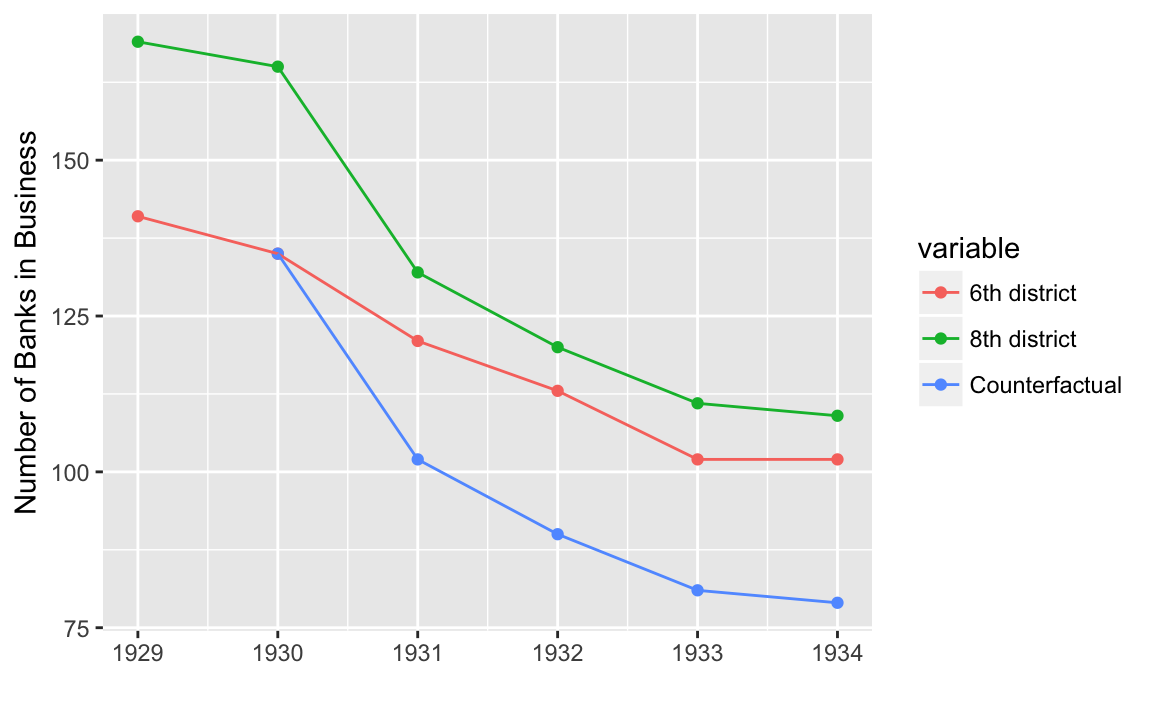
\includegraphics[width=0.7\linewidth]{banks_files/figure-latex/fig5.3-1} \end{center}

Plot the difference-in-difference estimate for all years after 1930.

\begin{Shaded}
\begin{Highlighting}[]
\KeywordTok{ggplot}\NormalTok{(}\KeywordTok{filter}\NormalTok{(banks, year }\OperatorTok{>}\StringTok{ }\DecValTok{1930}\NormalTok{), }\KeywordTok{aes}\NormalTok{(}\DataTypeTok{x =}\NormalTok{ year, }\DataTypeTok{y =}\NormalTok{ bib6 }\OperatorTok{-}\StringTok{ }\NormalTok{counterfactual)) }\OperatorTok{+}
\StringTok{  }\KeywordTok{geom_point}\NormalTok{() }\OperatorTok{+}
\StringTok{  }\KeywordTok{geom_line}\NormalTok{() }\OperatorTok{+}
\StringTok{  }\KeywordTok{ylab}\NormalTok{(}\StringTok{"DID (Number of Banks)"}\NormalTok{) }\OperatorTok{+}
\StringTok{  }\KeywordTok{xlab}\NormalTok{(}\StringTok{""}\NormalTok{)}
\end{Highlighting}
\end{Shaded}

\begin{figure}

{\centering 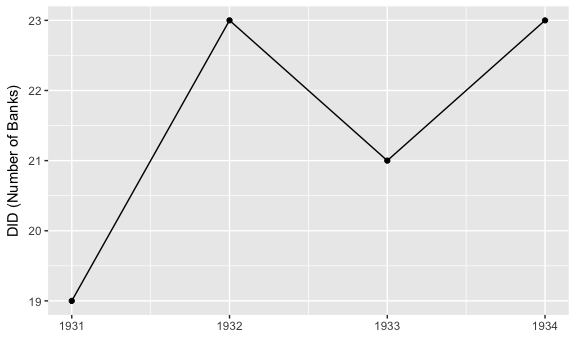
\includegraphics[width=0.7\linewidth]{banks_files/figure-latex/plot-bank-year-diff-1} 

}

\caption{Difference between Eighth District and Sixth District Counterfactuals}\label{fig:plot-bank-year-diff}
\end{figure}

\hypertarget{references-4}{%
\section{References}\label{references-4}}

\begin{itemize}
\tightlist
\item
  \url{http://masteringmetrics.com/wp-content/uploads/2015/02/master_banks.do}
\item
  \url{http://masteringmetrics.com/wp-content/uploads/2015/02/ReadMe_BankFailures.txt}
\end{itemize}

\hypertarget{mlda-difference-in-difference}{%
\chapter{MLDA
Difference-in-Difference}\label{mlda-difference-in-difference}}

Difference-in-difference estimates of the effect of the minimum legal
drinking age (MLDA) on mortality (Mouchel, Williams, and Zador 1987;
Norberg, Bierut, and Grucza 2009). This replicates the analyses in
Tables 5.2 and 5.3 in \emph{Mastering 'Metrics}.

Load necessary libraries.

\begin{Shaded}
\begin{Highlighting}[]
\KeywordTok{library}\NormalTok{(}\StringTok{"tidyverse"}\NormalTok{)}
\KeywordTok{library}\NormalTok{(}\StringTok{"haven"}\NormalTok{)}
\KeywordTok{library}\NormalTok{(}\StringTok{"rlang"}\NormalTok{)}
\KeywordTok{library}\NormalTok{(}\StringTok{"broom"}\NormalTok{)}
\KeywordTok{library}\NormalTok{(}\StringTok{"clubSandwich"}\NormalTok{)}
\end{Highlighting}
\end{Shaded}

\begin{Shaded}
\begin{Highlighting}[]
\KeywordTok{data}\NormalTok{(}\StringTok{"deaths"}\NormalTok{, }\DataTypeTok{package =} \StringTok{"masteringmetrics"}\NormalTok{)}
\end{Highlighting}
\end{Shaded}

In these regressions, we will use both indicator variables for year as
well as a trend, so make a factor version of the \texttt{year} variable.

\begin{Shaded}
\begin{Highlighting}[]
\NormalTok{deaths <-}\StringTok{ }\KeywordTok{mutate}\NormalTok{(deaths, }\DataTypeTok{year_fct =} \KeywordTok{factor}\NormalTok{(year))}
\end{Highlighting}
\end{Shaded}

\hypertarget{table-5.2}{%
\section{Table 5.2}\label{table-5.2}}

Regression DD Estimates of MLDA-Induced Deaths among 18-20 year-olds,
from 1970-1983

\begin{Shaded}
\begin{Highlighting}[]
\NormalTok{dtypes <-}\StringTok{ }\KeywordTok{c}\NormalTok{(}\StringTok{"all"}\NormalTok{ =}\StringTok{ "All deaths"}\NormalTok{,}
            \StringTok{"MVA"}\NormalTok{ =}\StringTok{ "Motor vehicle accidents"}\NormalTok{,}
            \StringTok{"suicide"}\NormalTok{ =}\StringTok{ "Suicide"}\NormalTok{,}
            \StringTok{"internal"}\NormalTok{ =}\StringTok{ "All internal causes"}\NormalTok{)}
\end{Highlighting}
\end{Shaded}

Estimate the DD for MLDA for all causes of death in 18-20 year olds. Run
the regression with \texttt{lm} and calculate the cluster robust
standard errors using \texttt{sandwich::vcovCL}. Subset the data.

\begin{Shaded}
\begin{Highlighting}[]
\NormalTok{data <-}\StringTok{ }\KeywordTok{filter}\NormalTok{(deaths, year }\OperatorTok{<=}\StringTok{ }\DecValTok{1983}\NormalTok{, agegr }\OperatorTok{==}\StringTok{ "18-20 yrs"}\NormalTok{, dtype }\OperatorTok{==}\StringTok{ "all"}\NormalTok{)}
\end{Highlighting}
\end{Shaded}

Run the OLS model.

\begin{Shaded}
\begin{Highlighting}[]
\NormalTok{mod <-}\StringTok{ }\KeywordTok{lm}\NormalTok{(mrate }\OperatorTok{~}\StringTok{ }\DecValTok{0} \OperatorTok{+}\StringTok{ }\NormalTok{legal }\OperatorTok{+}\StringTok{ }\NormalTok{state }\OperatorTok{+}\StringTok{ }\NormalTok{year_fct, }\DataTypeTok{data =}\NormalTok{ data)}
\end{Highlighting}
\end{Shaded}

Calculate cluster robust coefficients. These are calculated using a
different method than Stata uses, and thus will be slightly different
than those reported in the book.

\begin{Shaded}
\begin{Highlighting}[]
\NormalTok{vcov <-}\StringTok{ }\KeywordTok{vcovCR}\NormalTok{(mod, }\DataTypeTok{cluster =}\NormalTok{ data[[}\StringTok{"state"}\NormalTok{]],}
               \DataTypeTok{type =} \StringTok{"CR2"}\NormalTok{)}
\KeywordTok{coef_test}\NormalTok{(mod, }\DataTypeTok{vcov =}\NormalTok{ vcov) }\OperatorTok
\StringTok{  }\KeywordTok{rownames_to_column}\NormalTok{(}\DataTypeTok{var =} \StringTok{"term"}\NormalTok{) }\OperatorTok
\StringTok{  }\KeywordTok{as_tibble}\NormalTok{() }\OperatorTok
\StringTok{  }\KeywordTok{select}\NormalTok{(term, }\DataTypeTok{estimate =}\NormalTok{ beta, }\DataTypeTok{std.error =}\NormalTok{ SE) }\OperatorTok
\StringTok{  }\KeywordTok{filter}\NormalTok{(term }\OperatorTok{==}\StringTok{ "legal"}\NormalTok{) }\OperatorTok
\StringTok{  }\NormalTok{knitr}\OperatorTok{::}\KeywordTok{kable}\NormalTok{(}\DataTypeTok{digits =} \DecValTok{2}\NormalTok{)}
\end{Highlighting}
\end{Shaded}

\begin{tabular}{l|r|r}
\hline
term & estimate & std.error\\
\hline
legal & 10.8 & 4.48\\
\hline
\end{tabular}

Function to calculate clustered standard errors and return a tidy data
frame of the coefficients and standard errors.

\begin{Shaded}
\begin{Highlighting}[]
\NormalTok{cluster_se <-}\StringTok{ }\ControlFlowTok{function}\NormalTok{(mod, cluster, }\DataTypeTok{type =} \StringTok{"CR2"}\NormalTok{) \{}
\NormalTok{  vcov <-}\StringTok{ }\KeywordTok{vcovCR}\NormalTok{(mod, }\DataTypeTok{cluster =}\NormalTok{ cluster, }\DataTypeTok{type =} \StringTok{"CR2"}\NormalTok{)}
  \KeywordTok{coef_test}\NormalTok{(mod, }\DataTypeTok{vcov =}\NormalTok{ vcov) }\OperatorTok
\StringTok{    }\KeywordTok{rownames_to_column}\NormalTok{(}\DataTypeTok{var =} \StringTok{"term"}\NormalTok{) }\OperatorTok
\StringTok{    }\KeywordTok{as_tibble}\NormalTok{() }\OperatorTok
\StringTok{    }\KeywordTok{select}\NormalTok{(term, }\DataTypeTok{estimate =}\NormalTok{ beta, }\DataTypeTok{std.error =}\NormalTok{ SE)}
\NormalTok{\}}
\end{Highlighting}
\end{Shaded}

\begin{Shaded}
\begin{Highlighting}[]
\NormalTok{run_mlda_dd <-}\StringTok{ }\ControlFlowTok{function}\NormalTok{(i) \{}
\NormalTok{  data <-}\StringTok{ }\KeywordTok{filter}\NormalTok{(deaths, year }\OperatorTok{<=}\StringTok{ }\DecValTok{1983}\NormalTok{, agegr }\OperatorTok{==}\StringTok{ "18-20 yrs"}\NormalTok{, dtype }\OperatorTok{==}\StringTok{ }\NormalTok{i) }\CommentTok{# nolint}
\NormalTok{  mods <-}\StringTok{ }\KeywordTok{tribble}\NormalTok{(}
    \OperatorTok{~}\StringTok{ }\NormalTok{name, }\OperatorTok{~}\StringTok{ }\NormalTok{model,}
    \StringTok{"No trends, no weights"}\NormalTok{,}
    \KeywordTok{lm}\NormalTok{(mrate }\OperatorTok{~}\StringTok{ }\DecValTok{0} \OperatorTok{+}\StringTok{ }\NormalTok{legal }\OperatorTok{+}\StringTok{ }\NormalTok{state }\OperatorTok{+}\StringTok{ }\NormalTok{year_fct, }\DataTypeTok{data =}\NormalTok{ data),}
    \StringTok{"Time trends, no weights"}\NormalTok{,}
    \KeywordTok{lm}\NormalTok{(mrate }\OperatorTok{~}\StringTok{ }\DecValTok{0} \OperatorTok{+}\StringTok{ }\NormalTok{legal }\OperatorTok{+}\StringTok{ }\NormalTok{year_fct }\OperatorTok{+}\StringTok{ }\NormalTok{state }\OperatorTok{+}\StringTok{ }\NormalTok{state}\OperatorTok{:}\NormalTok{year, }\DataTypeTok{data =}\NormalTok{ data),}
    \StringTok{"No trends, weights"}\NormalTok{,}
    \KeywordTok{lm}\NormalTok{(mrate }\OperatorTok{~}\StringTok{ }\DecValTok{0} \OperatorTok{+}\StringTok{ }\NormalTok{legal }\OperatorTok{+}\StringTok{ }\NormalTok{year_fct }\OperatorTok{+}\StringTok{ }\NormalTok{state, }\DataTypeTok{data =}\NormalTok{ data, }\DataTypeTok{weights =}\NormalTok{ pop),}
    \CommentTok{# nolint start}
    \CommentTok{# "Time trends, weights",}
    \CommentTok{#   lm(mrate ~ 0 + legal + year_fct + state + state:year,}
    \CommentTok{#      data = data, weights = pop)}
    \CommentTok{# nolint end}
\NormalTok{  ) }\OperatorTok
\StringTok{    }\KeywordTok{mutate}\NormalTok{(}\DataTypeTok{coefs =} \KeywordTok{map}\NormalTok{(model, }\OperatorTok{~}\StringTok{ }\KeywordTok{cluster_se}\NormalTok{(.x, }\DataTypeTok{cluster =}\NormalTok{ data[[}\StringTok{"state"}\NormalTok{]],}
                                           \DataTypeTok{type =} \StringTok{"CR2"}\NormalTok{))) }\OperatorTok
\StringTok{    }\KeywordTok{unnest}\NormalTok{(coefs) }\OperatorTok
\StringTok{    }\KeywordTok{filter}\NormalTok{(term }\OperatorTok{==}\StringTok{ "legal"}\NormalTok{) }\OperatorTok
\StringTok{    }\KeywordTok{mutate}\NormalTok{(}\DataTypeTok{response =}\NormalTok{ i) }\OperatorTok
\StringTok{    }\KeywordTok{select}\NormalTok{(name, response, estimate, std.error)}
\NormalTok{\}}
\end{Highlighting}
\end{Shaded}

\begin{Shaded}
\begin{Highlighting}[]
\NormalTok{mlda_dd <-}\StringTok{ }\KeywordTok{map_df}\NormalTok{(}\KeywordTok{names}\NormalTok{(dtypes), run_mlda_dd)}
\end{Highlighting}
\end{Shaded}

\begin{Shaded}
\begin{Highlighting}[]
\NormalTok{mlda_dd }\OperatorTok
\StringTok{  }\NormalTok{knitr}\OperatorTok{::}\KeywordTok{kable}\NormalTok{(}\DataTypeTok{digits =} \DecValTok{2}\NormalTok{)}
\end{Highlighting}
\end{Shaded}

\begin{tabular}{l|l|r|r}
\hline
name & response & estimate & std.error\\
\hline
No trends, no weights & all & 10.80 & 4.48\\
\hline
Time trends, no weights & all & 8.47 & 4.74\\
\hline
No trends, weights & all & 12.41 & 4.78\\
\hline
No trends, no weights & MVA & 7.59 & 2.43\\
\hline
Time trends, no weights & MVA & 6.64 & 2.47\\
\hline
No trends, weights & MVA & 7.50 & 2.30\\
\hline
No trends, no weights & suicide & 0.59 & 0.57\\
\hline
Time trends, no weights & suicide & 0.47 & 0.74\\
\hline
No trends, weights & suicide & 1.49 & 0.92\\
\hline
No trends, no weights & internal & 1.33 & 1.53\\
\hline
Time trends, no weights & internal & 0.08 & 1.80\\
\hline
No trends, weights & internal & 1.89 & 1.83\\
\hline
\end{tabular}

\hypertarget{table-5.3}{%
\section{Table 5.3}\label{table-5.3}}

Regression DD Estimates of MLDA-Induced Deaths among 18-20 year-olds,
from 1970-1983, controlling for Beer Taxes. This is the analysis
presented in Angrist and Pischke (2014) Table 5.3.

\begin{Shaded}
\begin{Highlighting}[]
\NormalTok{run_beertax <-}\StringTok{ }\ControlFlowTok{function}\NormalTok{(i) \{}
\NormalTok{  data <-}\StringTok{ }\KeywordTok{filter}\NormalTok{(deaths, year }\OperatorTok{<=}\StringTok{ }\DecValTok{1983}\NormalTok{, agegr }\OperatorTok{==}\StringTok{ "18-20 yrs"}\NormalTok{,}
\NormalTok{                 dtype }\OperatorTok{==}\StringTok{ }\NormalTok{i, }\OperatorTok{!}\KeywordTok{is.na}\NormalTok{(beertaxa))}
\NormalTok{  out <-}\StringTok{ }\KeywordTok{tribble}\NormalTok{(}
    \OperatorTok{~}\StringTok{ }\NormalTok{name, }\OperatorTok{~}\StringTok{ }\NormalTok{model,}
    \StringTok{"No time trends"}\NormalTok{,}
    \KeywordTok{lm}\NormalTok{(mrate }\OperatorTok{~}\StringTok{ }\DecValTok{0} \OperatorTok{+}\StringTok{ }\NormalTok{legal }\OperatorTok{+}\StringTok{ }\NormalTok{beertaxa }\OperatorTok{+}\StringTok{ }\NormalTok{year_fct }\OperatorTok{+}\StringTok{ }\NormalTok{state, }\DataTypeTok{data =}\NormalTok{ data),}
    \StringTok{"Time trends"}\NormalTok{,}
    \KeywordTok{lm}\NormalTok{(mrate }\OperatorTok{~}\StringTok{ }\DecValTok{0} \OperatorTok{+}\StringTok{ }\NormalTok{legal }\OperatorTok{+}\StringTok{ }\NormalTok{beertaxa }\OperatorTok{+}\StringTok{ }\NormalTok{year_fct }\OperatorTok{+}\StringTok{ }\NormalTok{state }\OperatorTok{+}\StringTok{ }\NormalTok{state}\OperatorTok{:}\NormalTok{year,}
       \DataTypeTok{data =}\NormalTok{ data)}
\NormalTok{  ) }\OperatorTok
\StringTok{    }\CommentTok{# calc culstered standard errors}
\StringTok{    }\KeywordTok{mutate}\NormalTok{(}\DataTypeTok{coefs =} \KeywordTok{map}\NormalTok{(model, }\OperatorTok{~}\StringTok{ }\KeywordTok{cluster_se}\NormalTok{(.x, data[[}\StringTok{"state"}\NormalTok{]]))) }\OperatorTok
\StringTok{    }\KeywordTok{unnest}\NormalTok{(coefs) }\OperatorTok
\StringTok{    }\KeywordTok{filter}\NormalTok{(term }\OperatorTok\StringTok{ }\KeywordTok{c}\NormalTok{(}\StringTok{"legal"}\NormalTok{, }\StringTok{"beertaxa"}\NormalTok{)) }\OperatorTok
\StringTok{    }\KeywordTok{mutate}\NormalTok{(}\DataTypeTok{response =}\NormalTok{ i) }\OperatorTok
\StringTok{    }\KeywordTok{select}\NormalTok{(response, name, term, estimate, std.error)}
\NormalTok{\}}
\end{Highlighting}
\end{Shaded}

\begin{Shaded}
\begin{Highlighting}[]
\NormalTok{beertax <-}\StringTok{ }\KeywordTok{map_df}\NormalTok{(}\KeywordTok{names}\NormalTok{(dtypes), run_beertax)}
\end{Highlighting}
\end{Shaded}

\begin{Shaded}
\begin{Highlighting}[]
\NormalTok{beertax }\OperatorTok
\StringTok{  }\NormalTok{knitr}\OperatorTok{::}\KeywordTok{kable}\NormalTok{(}\DataTypeTok{digits =} \DecValTok{2}\NormalTok{)}
\end{Highlighting}
\end{Shaded}

\begin{tabular}{l|l|l|r|r}
\hline
response & name & term & estimate & std.error\\
\hline
all & No time trends & legal & 10.98 & 4.60\\
\hline
all & No time trends & beertaxa & 1.51 & 9.02\\
\hline
all & Time trends & legal & 10.03 & 4.57\\
\hline
all & Time trends & beertaxa & -5.52 & 30.40\\
\hline
MVA & No time trends & legal & 7.59 & 2.51\\
\hline
MVA & No time trends & beertaxa & 3.82 & 5.27\\
\hline
MVA & Time trends & legal & 6.89 & 2.47\\
\hline
MVA & Time trends & beertaxa & 26.88 & 18.76\\
\hline
suicide & No time trends & legal & 0.45 & 0.58\\
\hline
suicide & No time trends & beertaxa & -3.05 & 1.61\\
\hline
suicide & Time trends & legal & 0.38 & 0.72\\
\hline
suicide & Time trends & beertaxa & -12.13 & 8.28\\
\hline
internal & No time trends & legal & 1.46 & 1.56\\
\hline
internal & No time trends & beertaxa & -1.36 & 3.02\\
\hline
internal & Time trends & legal & 0.88 & 1.68\\
\hline
internal & Time trends & beertaxa & -10.31 & 10.90\\
\hline
\end{tabular}

\emph{Note:} I had trouble getting \texttt{sandwich::vcovCL} to estimate
clustered standard errors for this regression.

\hypertarget{references-5}{%
\section{References}\label{references-5}}

\begin{itemize}
\tightlist
\item
  \url{http://masteringmetrics.com/wp-content/uploads/2015/01/analysis.do}
\item
  \url{http://masteringmetrics.com/wp-content/uploads/2015/01/ReadMe_MLDA_DD.txt}
\end{itemize}

\hypertarget{part-chapter-6}{%
\part{Chapter 6}\label{part-chapter-6}}

\hypertarget{twins-and-returns-to-schooling}{%
\chapter{Twins and Returns to
Schooling}\label{twins-and-returns-to-schooling}}

Estimates of the returns to schooling for Twinsburg twins (Ashenfelter
and Krueger 1994; Ashenfelter and Rouse 1998). This replicates the
analysis in Table 6.2 of \emph{Mastering 'Metrics}.

\begin{Shaded}
\begin{Highlighting}[]
\KeywordTok{library}\NormalTok{(}\StringTok{"tidyverse"}\NormalTok{)}
\KeywordTok{library}\NormalTok{(}\StringTok{"sandwich"}\NormalTok{)}
\KeywordTok{library}\NormalTok{(}\StringTok{"lmtest"}\NormalTok{)}
\KeywordTok{library}\NormalTok{(}\StringTok{"AER"}\NormalTok{)}
\end{Highlighting}
\end{Shaded}

Load \texttt{twins} data.

\begin{Shaded}
\begin{Highlighting}[]
\KeywordTok{data}\NormalTok{(}\StringTok{"pubtwins"}\NormalTok{, }\DataTypeTok{package =} \StringTok{"masteringmetrics"}\NormalTok{)}
\end{Highlighting}
\end{Shaded}

Run a regression of log wage on controls (Column 1 of Table 6.2).

\begin{Shaded}
\begin{Highlighting}[]
\NormalTok{mod1 <-}\StringTok{ }\KeywordTok{lm}\NormalTok{(lwage }\OperatorTok{~}\StringTok{ }\NormalTok{educ }\OperatorTok{+}\StringTok{ }\KeywordTok{poly}\NormalTok{(age, }\DecValTok{2}\NormalTok{) }\OperatorTok{+}\StringTok{ }\NormalTok{female }\OperatorTok{+}\StringTok{ }\NormalTok{white, }\DataTypeTok{data =}\NormalTok{ pubtwins)}
\KeywordTok{coeftest}\NormalTok{(mod1, }\DataTypeTok{vcov =}\NormalTok{ sandwich)}
\CommentTok{#> }
\CommentTok{#> t test of coefficients:}
\CommentTok{#> }
\CommentTok{#>               Estimate Std. Error t value Pr(>|t|)    }
\CommentTok{#> (Intercept)     1.1791     0.1631    7.23  1.3e-12 ***}
\CommentTok{#> educ            0.1100     0.0104   10.54  < 2e-16 ***}
\CommentTok{#> poly(age, 2)1   4.9643     0.5697    8.71  < 2e-16 ***}
\CommentTok{#> poly(age, 2)2  -4.2957     0.5919   -7.26  1.1e-12 ***}
\CommentTok{#> female         -0.3180     0.0397   -8.00  5.4e-15 ***}
\CommentTok{#> white          -0.1001     0.0679   -1.47     0.14    }
\CommentTok{#> ---}
\CommentTok{#> Signif. codes:  0 '***' 0.001 '**' 0.01 '*' 0.05 '.' 0.1 ' ' 1}
\end{Highlighting}
\end{Shaded}

\emph{Note:} The \texttt{age} coefficients are different (but
equivalent) to those reported in the Table due to the the use of
\texttt{poly(age,\ .)}, which calculates orthogonal polynomials.

Run regression of the difference in log wage between twins on the
difference in education (Column 2 of Table 6.2).

\begin{Shaded}
\begin{Highlighting}[]
\NormalTok{mod2 <-}\StringTok{ }\KeywordTok{lm}\NormalTok{(dlwage }\OperatorTok{~}\StringTok{ }\NormalTok{deduc, }\DataTypeTok{data =} \KeywordTok{filter}\NormalTok{(pubtwins, first }\OperatorTok{==}\StringTok{ }\DecValTok{1}\NormalTok{))}
\KeywordTok{coeftest}\NormalTok{(mod2, }\DataTypeTok{vcov =}\NormalTok{ sandwich)}
\CommentTok{#> }
\CommentTok{#> t test of coefficients:}
\CommentTok{#> }
\CommentTok{#>             Estimate Std. Error t value Pr(>|t|)   }
\CommentTok{#> (Intercept)   0.0296     0.0275    1.07   0.2835   }
\CommentTok{#> deduc         0.0610     0.0198    3.09   0.0022 **}
\CommentTok{#> ---}
\CommentTok{#> Signif. codes:  0 '***' 0.001 '**' 0.01 '*' 0.05 '.' 0.1 ' ' 1}
\end{Highlighting}
\end{Shaded}

Run a regression of log wage on controls, instrumenting education with
twin's education (Column 3 of Table 6.2).

\begin{Shaded}
\begin{Highlighting}[]
\NormalTok{mod3 <-}\StringTok{ }\KeywordTok{ivreg}\NormalTok{(lwage }\OperatorTok{~}\StringTok{ }\NormalTok{educ }\OperatorTok{+}\StringTok{ }\KeywordTok{poly}\NormalTok{(age, }\DecValTok{2}\NormalTok{) }\OperatorTok{+}\StringTok{ }\NormalTok{female }\OperatorTok{+}\StringTok{ }\NormalTok{white }\OperatorTok{|}
\StringTok{                }\NormalTok{. }\OperatorTok{-}\StringTok{ }\NormalTok{educ }\OperatorTok{+}\StringTok{ }\NormalTok{educt, }\DataTypeTok{data =}\NormalTok{ pubtwins)}
\KeywordTok{summary}\NormalTok{(mod3, }\DataTypeTok{vcov =}\NormalTok{ sandwich, }\DataTypeTok{diagnostics =} \OtherTok{TRUE}\NormalTok{)}
\CommentTok{#> }
\CommentTok{#> Call:}
\CommentTok{#> ivreg(formula = lwage ~ educ + poly(age, 2) + female + white | }
\CommentTok{#>     . - educ + educt, data = pubtwins)}
\CommentTok{#> }
\CommentTok{#> Residuals:}
\CommentTok{#>      Min       1Q   Median       3Q      Max }
\CommentTok{#> -1.69585 -0.29218  0.00494  0.26262  2.47060 }
\CommentTok{#> }
\CommentTok{#> Coefficients:}
\CommentTok{#>               Estimate Std. Error t value Pr(>|t|)    }
\CommentTok{#> (Intercept)     1.0636     0.2113    5.03  6.2e-07 ***}
\CommentTok{#> educ            0.1179     0.0137    8.62  < 2e-16 ***}
\CommentTok{#> poly(age, 2)1   5.0367     0.5805    8.68  < 2e-16 ***}
\CommentTok{#> poly(age, 2)2  -4.2897     0.5928   -7.24  1.3e-12 ***}
\CommentTok{#> female         -0.3149     0.0403   -7.81  2.2e-14 ***}
\CommentTok{#> white          -0.0974     0.0682   -1.43     0.15    }
\CommentTok{#> }
\CommentTok{#> Diagnostic tests:}
\CommentTok{#>                  df1 df2 statistic p-value    }
\CommentTok{#> Weak instruments   1 674    796.30  <2e-16 ***}
\CommentTok{#> Wu-Hausman         1 673      0.92    0.34    }
\CommentTok{#> Sargan             0  NA        NA      NA    }
\CommentTok{#> ---}
\CommentTok{#> Signif. codes:  0 '***' 0.001 '**' 0.01 '*' 0.05 '.' 0.1 ' ' 1}
\CommentTok{#> }
\CommentTok{#> Residual standard error: 0.507 on 674 degrees of freedom}
\CommentTok{#> Multiple R-Squared: 0.338,   Adjusted R-squared: 0.333 }
\CommentTok{#> Wald test: 56.8 on 5 and 674 DF,  p-value: <2e-16}
\end{Highlighting}
\end{Shaded}

\emph{Note:} The coefficient for years of education is slightly
different than that reported in the book.

Run a regression of the difference in wage, instrumenting the difference
in years of education with twin's education (Column 4 of Table 6.2).

\begin{Shaded}
\begin{Highlighting}[]
\NormalTok{mod4 <-}\StringTok{ }\KeywordTok{ivreg}\NormalTok{(dlwage }\OperatorTok{~}\StringTok{ }\NormalTok{deduc }\OperatorTok{|}\StringTok{ }\NormalTok{deduct,}
              \DataTypeTok{data =} \KeywordTok{filter}\NormalTok{(pubtwins, first }\OperatorTok{==}\StringTok{ }\DecValTok{1}\NormalTok{))}
\KeywordTok{summary}\NormalTok{(mod4, }\DataTypeTok{vcov =}\NormalTok{ sandwich, }\DataTypeTok{diagnostics =} \OtherTok{TRUE}\NormalTok{)}
\CommentTok{#> }
\CommentTok{#> Call:}
\CommentTok{#> ivreg(formula = dlwage ~ deduc | deduct, data = filter(pubtwins, }
\CommentTok{#>     first == 1))}
\CommentTok{#> }
\CommentTok{#> Residuals:}
\CommentTok{#>     Min      1Q  Median      3Q     Max }
\CommentTok{#> -2.0423 -0.3111 -0.0274  0.2471  2.0824 }
\CommentTok{#> }
\CommentTok{#> Coefficients:}
\CommentTok{#>             Estimate Std. Error t value Pr(>|t|)   }
\CommentTok{#> (Intercept)   0.0274     0.0277    0.99   0.3237   }
\CommentTok{#> deduc         0.1070     0.0339    3.15   0.0018 **}
\CommentTok{#> }
\CommentTok{#> Diagnostic tests:}
\CommentTok{#>                  df1 df2 statistic p-value    }
\CommentTok{#> Weak instruments   1 338     85.15  <2e-16 ***}
\CommentTok{#> Wu-Hausman         1 337      4.12   0.043 *  }
\CommentTok{#> Sargan             0  NA        NA      NA    }
\CommentTok{#> ---}
\CommentTok{#> Signif. codes:  0 '***' 0.001 '**' 0.01 '*' 0.05 '.' 0.1 ' ' 1}
\CommentTok{#> }
\CommentTok{#> Residual standard error: 0.512 on 338 degrees of freedom}
\CommentTok{#> Multiple R-Squared: 0.0132,  Adjusted R-squared: 0.0103 }
\CommentTok{#> Wald test: 9.94 on 1 and 338 DF,  p-value: 0.00176}
\end{Highlighting}
\end{Shaded}

\emph{Note:} The coefficient for years of education is slightly
different than that reported in the book.

\hypertarget{references-6}{%
\section*{References}\label{references-6}}
\addcontentsline{toc}{section}{References}

\begin{itemize}
\tightlist
\item
  \url{http://masteringmetrics.com/wp-content/uploads/2015/02/ReadMe_Twinsburg.txt}
\item
  \url{http://masteringmetrics.com/wp-content/uploads/2015/02/twins.do}
\end{itemize}

\hypertarget{child-labor-laws-as-an-iv}{%
\chapter{Child Labor Laws as an IV}\label{child-labor-laws-as-an-iv}}

2SLS estimates of the returns to schooling using child labor laws as
instruments for years of schooling (Acemoglu and Angrist 2000). This
replicates Table 6.3 of \emph{Mastering 'Metrics}.

\begin{Shaded}
\begin{Highlighting}[]
\KeywordTok{library}\NormalTok{(}\StringTok{"AER"}\NormalTok{)}
\KeywordTok{library}\NormalTok{(}\StringTok{"sandwich"}\NormalTok{)}
\KeywordTok{library}\NormalTok{(}\StringTok{"clubSandwich"}\NormalTok{)}
\KeywordTok{library}\NormalTok{(}\StringTok{"tidyverse"}\NormalTok{)}
\KeywordTok{library}\NormalTok{(}\StringTok{"broom"}\NormalTok{)}
\end{Highlighting}
\end{Shaded}

Load the \texttt{child\_labor} data.

\begin{Shaded}
\begin{Highlighting}[]
\KeywordTok{data}\NormalTok{(}\StringTok{"child_labor"}\NormalTok{, }\DataTypeTok{package =} \StringTok{"masteringmetrics"}\NormalTok{)}
\NormalTok{child_labor <-}\StringTok{ }\KeywordTok{mutate}\NormalTok{(child_labor,}
                      \DataTypeTok{year =} \KeywordTok{factor}\NormalTok{(year),}
                      \DataTypeTok{yob_fct =} \KeywordTok{factor}\NormalTok{(yob),}
                      \DataTypeTok{sob =} \KeywordTok{factor}\NormalTok{(sob))}
\end{Highlighting}
\end{Shaded}

\hypertarget{first-stages-and-reduced-forms}{%
\section{First stages and reduced
forms}\label{first-stages-and-reduced-forms}}

Column 1. Years of Schooling.

\begin{Shaded}
\begin{Highlighting}[]
\NormalTok{mod1 <-}\StringTok{ }\KeywordTok{lm}\NormalTok{(indEduc }\OperatorTok{~}\StringTok{ }\NormalTok{year }\OperatorTok{+}\StringTok{ }\NormalTok{yob_fct }\OperatorTok{+}\StringTok{ }\NormalTok{sob }\OperatorTok{+}\StringTok{ }\NormalTok{cl7 }\OperatorTok{+}\StringTok{ }\NormalTok{cl8 }\OperatorTok{+}\StringTok{ }\NormalTok{cl9,}
           \DataTypeTok{data =}\NormalTok{ child_labor, }\DataTypeTok{weights =}\NormalTok{ weight)}
\CommentTok{# coef_test(mod1, vcov = vcovCR(mod1, cluster = child_labor[["sob"]]))}
\end{Highlighting}
\end{Shaded}

Column 2. Years of Schooling. State of birth dummies x linear year of
birth trends.

\begin{Shaded}
\begin{Highlighting}[]
\NormalTok{mod2 <-}\StringTok{ }\KeywordTok{lm}\NormalTok{(indEduc }\OperatorTok{~}\StringTok{ }\NormalTok{year }\OperatorTok{+}\StringTok{ }\NormalTok{yob_fct }\OperatorTok{+}\StringTok{ }\NormalTok{sob }\OperatorTok{+}\StringTok{ }\NormalTok{sob}\OperatorTok{:}\NormalTok{yob }\OperatorTok{+}\StringTok{ }\NormalTok{cl7 }\OperatorTok{+}\StringTok{ }\NormalTok{cl8 }\OperatorTok{+}\StringTok{ }\NormalTok{cl9,}
           \DataTypeTok{data =}\NormalTok{ child_labor, }\DataTypeTok{weights =}\NormalTok{ weight)}
\CommentTok{# coef_test(mod2, vcov = vcovCR(mod2, cluster = child_labor[["sob"]]))}
\end{Highlighting}
\end{Shaded}

Column 3. Log weekly wages.

\begin{Shaded}
\begin{Highlighting}[]
\NormalTok{mod3 <-}\StringTok{ }\KeywordTok{lm}\NormalTok{(lnwkwage }\OperatorTok{~}\StringTok{ }\NormalTok{year }\OperatorTok{+}\StringTok{ }\NormalTok{yob_fct }\OperatorTok{+}\StringTok{ }\NormalTok{sob }\OperatorTok{+}\StringTok{ }\NormalTok{cl7 }\OperatorTok{+}\StringTok{ }\NormalTok{cl8 }\OperatorTok{+}\StringTok{ }\NormalTok{cl9,}
           \DataTypeTok{data =}\NormalTok{ child_labor, }\DataTypeTok{weights =}\NormalTok{ weight)}
\CommentTok{# coef_test(mod3, vcov = vcovCR(mod1), cluster = child_labor[["state"]])}
\end{Highlighting}
\end{Shaded}

Column 4. Log weekly wages. State of birth dummies x linear year of
birth trends.

\begin{Shaded}
\begin{Highlighting}[]
\NormalTok{mod4 <-}\StringTok{ }\KeywordTok{lm}\NormalTok{(lnwkwage }\OperatorTok{~}\StringTok{ }\NormalTok{year }\OperatorTok{+}\StringTok{ }\NormalTok{yob_fct }\OperatorTok{+}\StringTok{ }\NormalTok{sob }\OperatorTok{+}\StringTok{ }\NormalTok{sob}\OperatorTok{:}\NormalTok{yob }\OperatorTok{+}\StringTok{ }\NormalTok{cl7 }\OperatorTok{+}\StringTok{ }\NormalTok{cl8 }\OperatorTok{+}\StringTok{ }\NormalTok{cl9,}
           \DataTypeTok{data =}\NormalTok{ child_labor, }\DataTypeTok{weights =}\NormalTok{ weight)}
\CommentTok{# coef_test(mod4, vcov = vcovCR(mod2), cluster = child_labor[["state"]])}
\end{Highlighting}
\end{Shaded}

\hypertarget{iv-returns}{%
\section{IV returns}\label{iv-returns}}

Column 3. Log weekly wages.

\begin{Shaded}
\begin{Highlighting}[]
\NormalTok{mod5 <-}\StringTok{ }\KeywordTok{ivreg}\NormalTok{(lnwkwage }\OperatorTok{~}\StringTok{ }\NormalTok{year }\OperatorTok{+}\StringTok{ }\NormalTok{yob_fct }\OperatorTok{+}\StringTok{ }\NormalTok{sob }\OperatorTok{+}\StringTok{ }\NormalTok{indEduc }\OperatorTok{|}
\StringTok{               }\NormalTok{. }\OperatorTok{-}\StringTok{ }\NormalTok{indEduc }\OperatorTok{+}\StringTok{ }\NormalTok{cl7 }\OperatorTok{+}\StringTok{ }\NormalTok{cl8 }\OperatorTok{+}\StringTok{ }\NormalTok{cl9,}
              \DataTypeTok{data =}\NormalTok{ child_labor, }\DataTypeTok{weights =}\NormalTok{ weight)}
\CommentTok{# coef_test(mod5, vcov = vcovCR(mod1), cluster = child_labor[["state"]])}
\end{Highlighting}
\end{Shaded}

Column 4. Log weekly wages. State of birth dummies x linear year of
birth trends.

\begin{Shaded}
\begin{Highlighting}[]
\NormalTok{mod6 <-}\StringTok{ }\KeywordTok{ivreg}\NormalTok{(lnwkwage }\OperatorTok{~}\StringTok{ }\NormalTok{year }\OperatorTok{+}\StringTok{ }\NormalTok{yob_fct }\OperatorTok{+}\StringTok{ }\NormalTok{sob }\OperatorTok{+}\StringTok{ }\NormalTok{sob}\OperatorTok{:}\NormalTok{yob }\OperatorTok{+}\StringTok{ }\NormalTok{indEduc }\OperatorTok{|}
\StringTok{               }\NormalTok{. }\OperatorTok{-}\StringTok{ }\NormalTok{indEduc }\OperatorTok{+}\StringTok{ }\NormalTok{cl7 }\OperatorTok{+}\StringTok{ }\NormalTok{cl8 }\OperatorTok{+}\StringTok{ }\NormalTok{cl9,}
              \DataTypeTok{data =}\NormalTok{ child_labor, }\DataTypeTok{weights =}\NormalTok{ weight)}
\CommentTok{# coef_test(mod6, vcov = vcovCR(mod2), cluster = child_labor[["state"]])}
\end{Highlighting}
\end{Shaded}

\hypertarget{references-7}{%
\section*{References}\label{references-7}}
\addcontentsline{toc}{section}{References}

\begin{itemize}
\tightlist
\item
  \url{http://masteringmetrics.com/wp-content/uploads/2015/02/ReadMe_ChildLaborLaws.txt}
\item
  \url{http://masteringmetrics.com/wp-content/uploads/2015/02/AA_regs.do}
\end{itemize}

\hypertarget{quarter-of-birth-and-returns-to-schooling}{%
\chapter{Quarter of Birth and Returns to
Schooling}\label{quarter-of-birth-and-returns-to-schooling}}

This replicates Tables 6.4 and 6.5, and Figures 6.1 and 6.2 of
\emph{Mastering 'Metrics}. These present an IV analysis of the returns
to schooling using quarters of birth (QOB) as instruments for years of
schooling (Angrist and Krueger 1991).

\begin{Shaded}
\begin{Highlighting}[]
\KeywordTok{library}\NormalTok{(}\StringTok{"AER"}\NormalTok{)}
\KeywordTok{library}\NormalTok{(}\StringTok{"sandwich"}\NormalTok{)}
\KeywordTok{library}\NormalTok{(}\StringTok{"lmtest"}\NormalTok{)}
\KeywordTok{library}\NormalTok{(}\StringTok{"tidyverse"}\NormalTok{)}
\KeywordTok{library}\NormalTok{(}\StringTok{"broom"}\NormalTok{)}
\end{Highlighting}
\end{Shaded}

Load \texttt{twins} data.

\begin{Shaded}
\begin{Highlighting}[]
\KeywordTok{data}\NormalTok{(}\StringTok{"ak91"}\NormalTok{, }\DataTypeTok{package =} \StringTok{"masteringmetrics"}\NormalTok{)}
\end{Highlighting}
\end{Shaded}

Some cleaning of the data.

\begin{Shaded}
\begin{Highlighting}[]
\NormalTok{ak91 <-}\StringTok{ }\KeywordTok{mutate}\NormalTok{(ak91,}
               \DataTypeTok{qob_fct =} \KeywordTok{factor}\NormalTok{(qob),}
               \DataTypeTok{q4 =} \KeywordTok{as.integer}\NormalTok{(qob }\OperatorTok{==}\StringTok{ "4"}\NormalTok{),}
               \DataTypeTok{yob_fct =} \KeywordTok{factor}\NormalTok{(yob))}
\end{Highlighting}
\end{Shaded}

Table 6.4. IV recipe for returns to schooling using a single QOB
instrument. Regress log wages on 4th quarter.

\begin{Shaded}
\begin{Highlighting}[]
\NormalTok{mod1 <-}\StringTok{ }\KeywordTok{lm}\NormalTok{(lnw }\OperatorTok{~}\StringTok{ }\NormalTok{q4, }\DataTypeTok{data =}\NormalTok{ ak91)}
\KeywordTok{coeftest}\NormalTok{(mod1, }\DataTypeTok{vcov =}\NormalTok{ sandwich)}
\CommentTok{#> }
\CommentTok{#> t test of coefficients:}
\CommentTok{#> }
\CommentTok{#>             Estimate Std. Error t value Pr(>|t|)    }
\CommentTok{#> (Intercept)  5.89827    0.00136 4329.13   <2e-16 ***}
\CommentTok{#> q4           0.00681    0.00274    2.48    0.013 *  }
\CommentTok{#> ---}
\CommentTok{#> Signif. codes:  0 '***' 0.001 '**' 0.01 '*' 0.05 '.' 0.1 ' ' 1}
\end{Highlighting}
\end{Shaded}

Regress years of schooling on 4th quarter.

\begin{Shaded}
\begin{Highlighting}[]
\NormalTok{mod2 <-}\StringTok{ }\KeywordTok{lm}\NormalTok{(s }\OperatorTok{~}\StringTok{ }\NormalTok{q4, }\DataTypeTok{data =}\NormalTok{ ak91)}
\KeywordTok{coeftest}\NormalTok{(mod2, }\DataTypeTok{vcov =}\NormalTok{ sandwich)}
\CommentTok{#> }
\CommentTok{#> t test of coefficients:}
\CommentTok{#> }
\CommentTok{#>             Estimate Std. Error t value Pr(>|t|)    }
\CommentTok{#> (Intercept) 12.74731    0.00661    1929  < 2e-16 ***}
\CommentTok{#> q4           0.09212    0.01316       7  2.6e-12 ***}
\CommentTok{#> ---}
\CommentTok{#> Signif. codes:  0 '***' 0.001 '**' 0.01 '*' 0.05 '.' 0.1 ' ' 1}
\end{Highlighting}
\end{Shaded}

IV regression of log wages on years of schooling, with 4th quarter as an
instrument for years of schooling.

\begin{Shaded}
\begin{Highlighting}[]
\NormalTok{mod3 <-}\StringTok{ }\KeywordTok{ivreg}\NormalTok{(lnw }\OperatorTok{~}\StringTok{ }\NormalTok{s }\OperatorTok{|}\StringTok{ }\NormalTok{q4, }\DataTypeTok{data =}\NormalTok{ ak91)}
\KeywordTok{coeftest}\NormalTok{(mod3, }\DataTypeTok{vcov =}\NormalTok{ sandwich)}
\CommentTok{#> }
\CommentTok{#> t test of coefficients:}
\CommentTok{#> }
\CommentTok{#>             Estimate Std. Error t value Pr(>|t|)    }
\CommentTok{#> (Intercept)    4.955      0.358   13.85   <2e-16 ***}
\CommentTok{#> s              0.074      0.028    2.64   0.0083 ** }
\CommentTok{#> ---}
\CommentTok{#> Signif. codes:  0 '***' 0.001 '**' 0.01 '*' 0.05 '.' 0.1 ' ' 1}
\end{Highlighting}
\end{Shaded}

\hypertarget{table-6.5}{%
\section{Table 6.5}\label{table-6.5}}

Regression Estimates of Returns to Schooling using Quarter of Birth
Instruments

Column 1. OLS

\begin{Shaded}
\begin{Highlighting}[]
\NormalTok{mod4 <-}\StringTok{ }\KeywordTok{lm}\NormalTok{(lnw }\OperatorTok{~}\StringTok{ }\NormalTok{s, }\DataTypeTok{data =}\NormalTok{ ak91)}
\KeywordTok{coeftest}\NormalTok{(mod4, }\DataTypeTok{vcov =}\NormalTok{ sandwich)}
\CommentTok{#> }
\CommentTok{#> t test of coefficients:}
\CommentTok{#> }
\CommentTok{#>             Estimate Std. Error t value Pr(>|t|)    }
\CommentTok{#> (Intercept) 4.995182   0.005074     984   <2e-16 ***}
\CommentTok{#> s           0.070851   0.000381     186   <2e-16 ***}
\CommentTok{#> ---}
\CommentTok{#> Signif. codes:  0 '***' 0.001 '**' 0.01 '*' 0.05 '.' 0.1 ' ' 1}
\end{Highlighting}
\end{Shaded}

Column 2. IV with only the 4th quarter as an instrument.

\begin{Shaded}
\begin{Highlighting}[]
\NormalTok{mod5 <-}\StringTok{ }\KeywordTok{ivreg}\NormalTok{(lnw }\OperatorTok{~}\StringTok{ }\NormalTok{s }\OperatorTok{|}\StringTok{ }\NormalTok{q4, }\DataTypeTok{data =}\NormalTok{ ak91)}
\KeywordTok{summary}\NormalTok{(mod5, }\DataTypeTok{vcov =}\NormalTok{ sandwich, }\DataTypeTok{diagnostics =} \OtherTok{TRUE}\NormalTok{)}
\CommentTok{#> }
\CommentTok{#> Call:}
\CommentTok{#> ivreg(formula = lnw ~ s | q4, data = ak91)}
\CommentTok{#> }
\CommentTok{#> Residuals:}
\CommentTok{#>     Min      1Q  Median      3Q     Max }
\CommentTok{#> -8.7765 -0.2393  0.0713  0.3326  4.6536 }
\CommentTok{#> }
\CommentTok{#> Coefficients:}
\CommentTok{#>             Estimate Std. Error t value Pr(>|t|)    }
\CommentTok{#> (Intercept)    4.955      0.358   13.85   <2e-16 ***}
\CommentTok{#> s              0.074      0.028    2.64   0.0083 ** }
\CommentTok{#> }
\CommentTok{#> Diagnostic tests:}
\CommentTok{#>                     df1    df2 statistic p-value    }
\CommentTok{#> Weak instruments      1 329507     48.99 2.6e-12 ***}
\CommentTok{#> Wu-Hausman            1 329506      0.01    0.91    }
\CommentTok{#> Sargan                0     NA        NA      NA    }
\CommentTok{#> ---}
\CommentTok{#> Signif. codes:  0 '***' 0.001 '**' 0.01 '*' 0.05 '.' 0.1 ' ' 1}
\CommentTok{#> }
\CommentTok{#> Residual standard error: 0.638 on 329507 degrees of freedom}
\CommentTok{#> Multiple R-Squared: 0.117,   Adjusted R-squared: 0.117 }
\CommentTok{#> Wald test: 6.97 on 1 and 329507 DF,  p-value: 0.00829}
\end{Highlighting}
\end{Shaded}

The argument \texttt{diagnostics\ =\ TRUE} will run an F-test on the
first stage which is reported as the ``Weak instruments'' diagnostic.

Column 3. OLS. Controls for year of birth.

\begin{Shaded}
\begin{Highlighting}[]
\NormalTok{mod6 <-}\StringTok{ }\KeywordTok{lm}\NormalTok{(lnw }\OperatorTok{~}\StringTok{ }\NormalTok{s }\OperatorTok{+}\StringTok{ }\NormalTok{yob_fct, }\DataTypeTok{data =}\NormalTok{ ak91)}
\KeywordTok{coeftest}\NormalTok{(mod6, }\DataTypeTok{vcov =}\NormalTok{ sandwich)}
\CommentTok{#> }
\CommentTok{#> t test of coefficients:}
\CommentTok{#> }
\CommentTok{#>              Estimate Std. Error t value Pr(>|t|)    }
\CommentTok{#> (Intercept)  5.017348   0.006019  833.65  < 2e-16 ***}
\CommentTok{#> s            0.071081   0.000381  186.34  < 2e-16 ***}
\CommentTok{#> yob_fct31   -0.006387   0.005123   -1.25  0.21251    }
\CommentTok{#> yob_fct32   -0.014838   0.005052   -2.94  0.00331 ** }
\CommentTok{#> yob_fct33   -0.017583   0.005068   -3.47  0.00052 ***}
\CommentTok{#> yob_fct34   -0.020999   0.005062   -4.15  3.3e-05 ***}
\CommentTok{#> yob_fct35   -0.032895   0.005039   -6.53  6.7e-11 ***}
\CommentTok{#> yob_fct36   -0.031781   0.004970   -6.39  1.6e-10 ***}
\CommentTok{#> yob_fct37   -0.036712   0.004894   -7.50  6.4e-14 ***}
\CommentTok{#> yob_fct38   -0.036890   0.004856   -7.60  3.1e-14 ***}
\CommentTok{#> yob_fct39   -0.048164   0.004833   -9.96  < 2e-16 ***}
\CommentTok{#> ---}
\CommentTok{#> Signif. codes:  0 '***' 0.001 '**' 0.01 '*' 0.05 '.' 0.1 ' ' 1}
\end{Highlighting}
\end{Shaded}

Column 4. IV reg using only the 4th quarter as an instrument. Controls
for year of birth.

\begin{Shaded}
\begin{Highlighting}[]
\NormalTok{mod7 <-}\StringTok{ }\KeywordTok{ivreg}\NormalTok{(lnw }\OperatorTok{~}\StringTok{ }\NormalTok{s }\OperatorTok{+}\StringTok{ }\NormalTok{yob_fct }\OperatorTok{|}\StringTok{ }\NormalTok{q4 }\OperatorTok{+}\StringTok{ }\NormalTok{yob_fct, }\DataTypeTok{data =}\NormalTok{ ak91)}
\KeywordTok{summary}\NormalTok{(mod7, }\DataTypeTok{vcov =}\NormalTok{ sandwich, }\DataTypeTok{diagnostics =} \OtherTok{TRUE}\NormalTok{)}
\CommentTok{#> }
\CommentTok{#> Call:}
\CommentTok{#> ivreg(formula = lnw ~ s + yob_fct | q4 + yob_fct, data = ak91)}
\CommentTok{#> }
\CommentTok{#> Residuals:}
\CommentTok{#>     Min      1Q  Median      3Q     Max }
\CommentTok{#> -8.7785 -0.2346  0.0719  0.3405  4.6687 }
\CommentTok{#> }
\CommentTok{#> Coefficients:}
\CommentTok{#>             Estimate Std. Error t value Pr(>|t|)    }
\CommentTok{#> (Intercept)  4.96599    0.35393   14.03   <2e-16 ***}
\CommentTok{#> s            0.07520    0.02841    2.65   0.0081 ** }
\CommentTok{#> yob_fct31   -0.00696    0.00647   -1.08   0.2819    }
\CommentTok{#> yob_fct32   -0.01557    0.00708   -2.20   0.0279 *  }
\CommentTok{#> yob_fct33   -0.01855    0.00833   -2.23   0.0259 *  }
\CommentTok{#> yob_fct34   -0.02209    0.00909   -2.43   0.0151 *  }
\CommentTok{#> yob_fct35   -0.03425    0.01061   -3.23   0.0012 ** }
\CommentTok{#> yob_fct36   -0.03338    0.01208   -2.76   0.0057 ** }
\CommentTok{#> yob_fct37   -0.03857    0.01368   -2.82   0.0048 ** }
\CommentTok{#> yob_fct38   -0.03910    0.01596   -2.45   0.0143 *  }
\CommentTok{#> yob_fct39   -0.05053    0.01705   -2.96   0.0030 ** }
\CommentTok{#> }
\CommentTok{#> Diagnostic tests:}
\CommentTok{#>                     df1    df2 statistic p-value    }
\CommentTok{#> Weak instruments      1 329498     47.73 4.9e-12 ***}
\CommentTok{#> Wu-Hausman            1 329497      0.02    0.88    }
\CommentTok{#> Sargan                0     NA        NA      NA    }
\CommentTok{#> ---}
\CommentTok{#> Signif. codes:  0 '***' 0.001 '**' 0.01 '*' 0.05 '.' 0.1 ' ' 1}
\CommentTok{#> }
\CommentTok{#> Residual standard error: 0.638 on 329498 degrees of freedom}
\CommentTok{#> Multiple R-Squared: 0.117,   Adjusted R-squared: 0.117 }
\CommentTok{#> Wald test: 1.81 on 10 and 329498 DF,  p-value: 0.054}
\end{Highlighting}
\end{Shaded}

Column 4. IV reg using all quarters as instruments. Controls for year of
birth.

\begin{Shaded}
\begin{Highlighting}[]
\NormalTok{mod8 <-}\StringTok{ }\KeywordTok{ivreg}\NormalTok{(lnw }\OperatorTok{~}\StringTok{ }\NormalTok{s }\OperatorTok{+}\StringTok{ }\NormalTok{yob_fct }\OperatorTok{|}\StringTok{ }\NormalTok{qob_fct }\OperatorTok{+}\StringTok{ }\NormalTok{yob_fct, }\DataTypeTok{data =}\NormalTok{ ak91)}
\KeywordTok{summary}\NormalTok{(mod8, }\DataTypeTok{vcov =}\NormalTok{ sandwich, }\DataTypeTok{diagnostics =} \OtherTok{TRUE}\NormalTok{)}
\CommentTok{#> }
\CommentTok{#> Call:}
\CommentTok{#> ivreg(formula = lnw ~ s + yob_fct | qob_fct + yob_fct, data = ak91)}
\CommentTok{#> }
\CommentTok{#> Residuals:}
\CommentTok{#>     Min      1Q  Median      3Q     Max }
\CommentTok{#> -8.9945 -0.2544  0.0676  0.3509  4.8425 }
\CommentTok{#> }
\CommentTok{#> Coefficients:}
\CommentTok{#>             Estimate Std. Error t value Pr(>|t|)    }
\CommentTok{#> (Intercept)  4.59174    0.25057   18.32  < 2e-16 ***}
\CommentTok{#> s            0.10525    0.02012    5.23  1.7e-07 ***}
\CommentTok{#> yob_fct31   -0.01111    0.00591   -1.88  0.05988 .  }
\CommentTok{#> yob_fct32   -0.02089    0.00623   -3.35  0.00080 ***}
\CommentTok{#> yob_fct33   -0.02556    0.00698   -3.66  0.00025 ***}
\CommentTok{#> yob_fct34   -0.03007    0.00742   -4.05  5.1e-05 ***}
\CommentTok{#> yob_fct35   -0.04414    0.00836   -5.28  1.3e-07 ***}
\CommentTok{#> yob_fct36   -0.04501    0.00930   -4.84  1.3e-06 ***}
\CommentTok{#> yob_fct37   -0.05207    0.01034   -5.04  4.7e-07 ***}
\CommentTok{#> yob_fct38   -0.05518    0.01184   -4.66  3.1e-06 ***}
\CommentTok{#> yob_fct39   -0.06780    0.01259   -5.39  7.2e-08 ***}
\CommentTok{#> }
\CommentTok{#> Diagnostic tests:}
\CommentTok{#>                     df1    df2 statistic p-value    }
\CommentTok{#> Weak instruments      3 329496     32.32  <2e-16 ***}
\CommentTok{#> Wu-Hausman            1 329497      2.98   0.084 .  }
\CommentTok{#> Sargan                2     NA      3.26   0.196    }
\CommentTok{#> ---}
\CommentTok{#> Signif. codes:  0 '***' 0.001 '**' 0.01 '*' 0.05 '.' 0.1 ' ' 1}
\CommentTok{#> }
\CommentTok{#> Residual standard error: 0.647 on 329498 degrees of freedom}
\CommentTok{#> Multiple R-Squared: 0.0905,  Adjusted R-squared: 0.0905 }
\CommentTok{#> Wald test: 3.79 on 10 and 329498 DF,  p-value: 3.9e-05}
\end{Highlighting}
\end{Shaded}

\hypertarget{figures}{%
\section{Figures}\label{figures}}

Summarize the average wages by age:

\begin{Shaded}
\begin{Highlighting}[]
\NormalTok{ak91_age <-}\StringTok{ }\NormalTok{ak91 }\OperatorTok
\StringTok{  }\KeywordTok{group_by}\NormalTok{(qob, yob) }\OperatorTok
\StringTok{  }\KeywordTok{summarise}\NormalTok{(}\DataTypeTok{lnw =} \KeywordTok{mean}\NormalTok{(lnw), }\DataTypeTok{s =} \KeywordTok{mean}\NormalTok{(s)) }\OperatorTok
\StringTok{  }\KeywordTok{mutate}\NormalTok{(}\DataTypeTok{q4 =}\NormalTok{ (qob }\OperatorTok{==}\StringTok{ }\DecValTok{4}\NormalTok{))}
\end{Highlighting}
\end{Shaded}

Average years of schooling by quarter of birth for men born in 1930-39
in the 1980 US Census.

\begin{Shaded}
\begin{Highlighting}[]
\KeywordTok{ggplot}\NormalTok{(ak91_age, }\KeywordTok{aes}\NormalTok{(}\DataTypeTok{x =}\NormalTok{ yob }\OperatorTok{+}\StringTok{ }\NormalTok{(qob }\OperatorTok{-}\StringTok{ }\DecValTok{1}\NormalTok{) }\OperatorTok{/}\StringTok{ }\DecValTok{4}\NormalTok{, }\DataTypeTok{y =}\NormalTok{ s)) }\OperatorTok{+}
\StringTok{  }\KeywordTok{geom_line}\NormalTok{() }\OperatorTok{+}
\StringTok{  }\KeywordTok{geom_label}\NormalTok{(}\DataTypeTok{mapping =} \KeywordTok{aes}\NormalTok{(}\DataTypeTok{label =}\NormalTok{ qob, }\DataTypeTok{color =}\NormalTok{ q4)) }\OperatorTok{+}
\StringTok{  }\KeywordTok{theme}\NormalTok{(}\DataTypeTok{legend.position =} \StringTok{"none"}\NormalTok{) }\OperatorTok{+}
\StringTok{  }\KeywordTok{scale_x_continuous}\NormalTok{(}\StringTok{"Year of birth"}\NormalTok{, }\DataTypeTok{breaks =} \DecValTok{1930}\OperatorTok{:}\DecValTok{1940}\NormalTok{) }\OperatorTok{+}
\StringTok{  }\KeywordTok{scale_y_continuous}\NormalTok{(}\StringTok{"Years of Education"}\NormalTok{, }\DataTypeTok{breaks =} \KeywordTok{seq}\NormalTok{(}\FloatTok{12.2}\NormalTok{, }\FloatTok{13.2}\NormalTok{, }\DataTypeTok{by =} \FloatTok{0.2}\NormalTok{),}
                     \DataTypeTok{limits =} \KeywordTok{c}\NormalTok{(}\FloatTok{12.2}\NormalTok{, }\FloatTok{13.2}\NormalTok{))}
\end{Highlighting}
\end{Shaded}

\begin{center}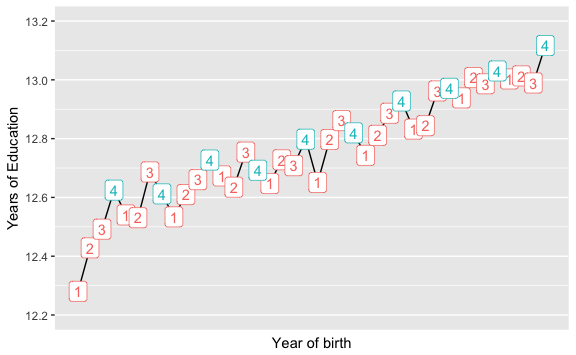
\includegraphics[width=0.7\linewidth]{ak91_files/figure-latex/unnamed-chunk-8-1} \end{center}

Average log wages by quarter of birth for men born in 1930-39 in the
1980 US Census.

\begin{Shaded}
\begin{Highlighting}[]
\KeywordTok{ggplot}\NormalTok{(ak91_age, }\KeywordTok{aes}\NormalTok{(}\DataTypeTok{x =}\NormalTok{ yob }\OperatorTok{+}\StringTok{ }\NormalTok{(qob }\OperatorTok{-}\StringTok{ }\DecValTok{1}\NormalTok{) }\OperatorTok{/}\StringTok{ }\DecValTok{4}\NormalTok{, }\DataTypeTok{y =}\NormalTok{ lnw)) }\OperatorTok{+}
\StringTok{  }\KeywordTok{geom_line}\NormalTok{() }\OperatorTok{+}
\StringTok{  }\KeywordTok{geom_label}\NormalTok{(}\DataTypeTok{mapping =} \KeywordTok{aes}\NormalTok{(}\DataTypeTok{label =}\NormalTok{ qob, }\DataTypeTok{color =}\NormalTok{ q4)) }\OperatorTok{+}
\StringTok{  }\KeywordTok{scale_x_continuous}\NormalTok{(}\StringTok{"Year of birth"}\NormalTok{, }\DataTypeTok{breaks =} \DecValTok{1930}\OperatorTok{:}\DecValTok{1940}\NormalTok{) }\OperatorTok{+}
\StringTok{  }\KeywordTok{scale_y_continuous}\NormalTok{(}\StringTok{"Log weekly wages"}\NormalTok{) }\OperatorTok{+}
\StringTok{  }\KeywordTok{theme}\NormalTok{(}\DataTypeTok{legend.position =} \StringTok{"none"}\NormalTok{)}
\end{Highlighting}
\end{Shaded}

\begin{center}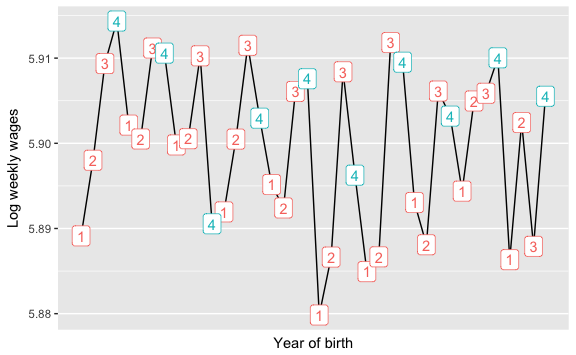
\includegraphics[width=0.7\linewidth]{ak91_files/figure-latex/unnamed-chunk-9-1} \end{center}

\hypertarget{references-8}{%
\section*{References}\label{references-8}}
\addcontentsline{toc}{section}{References}

\begin{itemize}
\tightlist
\item
  \url{http://masteringmetrics.com/wp-content/uploads/2015/02/ReadMe_QOB.txt}
\item
  \url{http://masteringmetrics.com/wp-content/uploads/2015/02/ak91.do}
\end{itemize}

\hypertarget{sheepskin-and-returns-to-schooling}{%
\chapter{Sheepskin and Returns to
Schooling}\label{sheepskin-and-returns-to-schooling}}

This replicates Figures 6.3 and 6.4 of \emph{Mastering 'Metrics}. These
analyses use a fuzzy RD design to analyze the ``sheepskin effects'' of a
high school diploma (Clark and Martorell 2014).

\begin{Shaded}
\begin{Highlighting}[]
\KeywordTok{library}\NormalTok{(}\StringTok{"tidyverse"}\NormalTok{)}
\end{Highlighting}
\end{Shaded}

Load \texttt{sheepskin} data.

\begin{Shaded}
\begin{Highlighting}[]
\KeywordTok{data}\NormalTok{(}\StringTok{"sheepskin"}\NormalTok{, }\DataTypeTok{package =} \StringTok{"masteringmetrics"}\NormalTok{)}
\end{Highlighting}
\end{Shaded}

Create indicator variable for passing the test.

\begin{Shaded}
\begin{Highlighting}[]
\NormalTok{sheepskin <-}\StringTok{ }\KeywordTok{mutate}\NormalTok{(sheepskin, }\DataTypeTok{test_lcs_pass =}\NormalTok{ (minscore }\OperatorTok{>=}\StringTok{ }\DecValTok{0}\NormalTok{))}
\end{Highlighting}
\end{Shaded}

\hypertarget{figure-1}{%
\section{Figure 1}\label{figure-1}}

Figure 1. Regression discontinuity

\begin{Shaded}
\begin{Highlighting}[]
\NormalTok{mod1_lhs <-}\StringTok{ }\KeywordTok{lm}\NormalTok{(receivehsd }\OperatorTok{~}\StringTok{ }\KeywordTok{poly}\NormalTok{(minscore, }\DecValTok{4}\NormalTok{),}
               \DataTypeTok{data =} \KeywordTok{filter}\NormalTok{(sheepskin, minscore }\OperatorTok{<}\StringTok{ }\DecValTok{0}\NormalTok{), }\DataTypeTok{weights =}\NormalTok{ n)}
\NormalTok{mod1_rhs <-}\StringTok{ }\KeywordTok{lm}\NormalTok{(receivehsd }\OperatorTok{~}\StringTok{ }\KeywordTok{poly}\NormalTok{(minscore, }\DecValTok{4}\NormalTok{),}
               \DataTypeTok{data =} \KeywordTok{filter}\NormalTok{(sheepskin, minscore }\OperatorTok{>=}\StringTok{ }\DecValTok{0}\NormalTok{), }\DataTypeTok{weights =}\NormalTok{ n)}
\end{Highlighting}
\end{Shaded}

Append fitted values to the original dataset

\begin{Shaded}
\begin{Highlighting}[]
\NormalTok{fig1_data <-}\StringTok{ }\NormalTok{sheepskin }\OperatorTok
\StringTok{  }\KeywordTok{select}\NormalTok{(minscore, receivehsd, n) }\OperatorTok
\StringTok{  }\NormalTok{modelr}\OperatorTok{::}\KeywordTok{add_predictions}\NormalTok{(mod1_lhs, }\DataTypeTok{var =} \StringTok{"fit_hsd2_l"}\NormalTok{) }\OperatorTok
\StringTok{  }\KeywordTok{mutate}\NormalTok{(}\DataTypeTok{fit_hsd2_l =} \KeywordTok{if_else}\NormalTok{(minscore }\OperatorTok{>}\StringTok{ }\DecValTok{0}\NormalTok{, }\OtherTok{NA_real_}\NormalTok{, fit_hsd2_l)) }\OperatorTok
\StringTok{  }\NormalTok{modelr}\OperatorTok{::}\KeywordTok{add_predictions}\NormalTok{(mod1_rhs, }\DataTypeTok{var =} \StringTok{"fit_hsd2_r"}\NormalTok{) }\OperatorTok
\StringTok{  }\KeywordTok{mutate}\NormalTok{(}\DataTypeTok{fit_hsd2_r =} \KeywordTok{if_else}\NormalTok{(minscore }\OperatorTok{<}\StringTok{ }\DecValTok{0}\NormalTok{, }\OtherTok{NA_real_}\NormalTok{, fit_hsd2_r))}
\end{Highlighting}
\end{Shaded}

Figure 6.3.

\begin{Shaded}
\begin{Highlighting}[]
\KeywordTok{ggplot}\NormalTok{(fig1_data, }\KeywordTok{aes}\NormalTok{(}\DataTypeTok{x =}\NormalTok{ minscore)) }\OperatorTok{+}
\StringTok{  }\KeywordTok{geom_vline}\NormalTok{(}\DataTypeTok{xintercept =} \DecValTok{0}\NormalTok{, }\DataTypeTok{color =} \StringTok{"white"}\NormalTok{, }\DataTypeTok{size =} \DecValTok{2}\NormalTok{) }\OperatorTok{+}
\StringTok{  }\KeywordTok{geom_point}\NormalTok{(}\DataTypeTok{mapping =} \KeywordTok{aes}\NormalTok{(}\DataTypeTok{y =}\NormalTok{ receivehsd), }\DataTypeTok{color =} \StringTok{"gray"}\NormalTok{) }\OperatorTok{+}
\StringTok{  }\KeywordTok{geom_line}\NormalTok{(}\DataTypeTok{mapping =} \KeywordTok{aes}\NormalTok{(}\DataTypeTok{y =}\NormalTok{ fit_hsd2_l)) }\OperatorTok{+}
\StringTok{  }\KeywordTok{geom_line}\NormalTok{(}\DataTypeTok{mapping =} \KeywordTok{aes}\NormalTok{(}\DataTypeTok{y =}\NormalTok{ fit_hsd2_r)) }\OperatorTok{+}
\StringTok{  }\KeywordTok{scale_x_continuous}\NormalTok{(}\StringTok{"Test Scores Relative to Cutoff"}\NormalTok{,}
                     \DataTypeTok{breaks =} \KeywordTok{seq}\NormalTok{(}\OperatorTok{-}\DecValTok{30}\NormalTok{, }\DecValTok{15}\NormalTok{, }\DataTypeTok{by =} \DecValTok{5}\NormalTok{), }\DataTypeTok{limits =} \KeywordTok{c}\NormalTok{(}\OperatorTok{-}\DecValTok{30}\NormalTok{, }\DecValTok{15}\NormalTok{)) }\OperatorTok{+}
\StringTok{  }\KeywordTok{scale_y_continuous}\NormalTok{(}\StringTok{"Fraction Receiving Diplomas"}\NormalTok{,}
                     \DataTypeTok{breaks =} \KeywordTok{seq}\NormalTok{(}\DecValTok{0}\NormalTok{, }\DecValTok{1}\NormalTok{, }\DataTypeTok{by =} \FloatTok{0.2}\NormalTok{), }\DataTypeTok{limits =} \KeywordTok{c}\NormalTok{(}\DecValTok{0}\NormalTok{, }\DecValTok{1}\NormalTok{))}
\end{Highlighting}
\end{Shaded}

\begin{figure}

{\centering 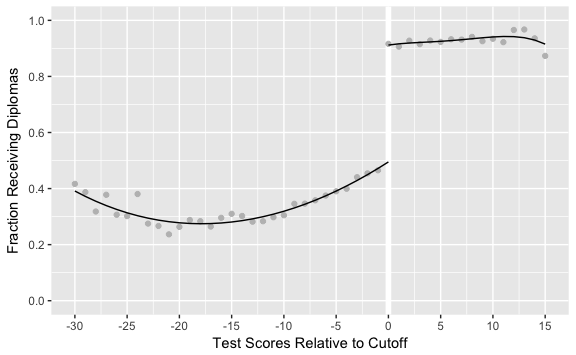
\includegraphics[width=0.7\linewidth]{sheepskin_files/figure-latex/fig.6.3-1} 

}

\caption{Last-chance exams and Texas sheepskin}(\#fig:fig.6.3)
\end{figure}

\hypertarget{figure-2}{%
\section{Figure 2}\label{figure-2}}

\begin{Shaded}
\begin{Highlighting}[]
\NormalTok{mod2_lhs <-}\StringTok{ }\KeywordTok{lm}\NormalTok{(avgearnings }\OperatorTok{~}\StringTok{ }\KeywordTok{poly}\NormalTok{(minscore, }\DecValTok{4}\NormalTok{),}
               \DataTypeTok{data =} \KeywordTok{filter}\NormalTok{(sheepskin, minscore }\OperatorTok{<}\StringTok{ }\DecValTok{0}\NormalTok{),}
               \DataTypeTok{weights =}\NormalTok{ n)}
\NormalTok{mod2_rhs <-}\StringTok{ }\KeywordTok{lm}\NormalTok{(avgearnings }\OperatorTok{~}\StringTok{ }\KeywordTok{poly}\NormalTok{(minscore, }\DecValTok{4}\NormalTok{),}
               \DataTypeTok{data =} \KeywordTok{filter}\NormalTok{(sheepskin, minscore }\OperatorTok{>=}\StringTok{ }\DecValTok{0}\NormalTok{), }\DataTypeTok{weights =}\NormalTok{ n)}
\end{Highlighting}
\end{Shaded}

Append fitted values to the original dataset

\begin{Shaded}
\begin{Highlighting}[]
\NormalTok{fig2_data <-}\StringTok{ }\NormalTok{sheepskin }\OperatorTok
\StringTok{  }\KeywordTok{select}\NormalTok{(minscore, avgearnings, n) }\OperatorTok
\StringTok{  }\NormalTok{modelr}\OperatorTok{::}\KeywordTok{add_predictions}\NormalTok{(mod2_lhs, }\DataTypeTok{var =} \StringTok{"fit_l"}\NormalTok{) }\OperatorTok
\StringTok{  }\KeywordTok{mutate}\NormalTok{(}\DataTypeTok{fit_l =} \KeywordTok{if_else}\NormalTok{(minscore }\OperatorTok{>}\StringTok{ }\DecValTok{0}\NormalTok{, }\OtherTok{NA_real_}\NormalTok{, fit_l)) }\OperatorTok
\StringTok{  }\NormalTok{modelr}\OperatorTok{::}\KeywordTok{add_predictions}\NormalTok{(mod2_rhs, }\DataTypeTok{var =} \StringTok{"fit_r"}\NormalTok{) }\OperatorTok
\StringTok{  }\KeywordTok{mutate}\NormalTok{(}\DataTypeTok{fit_r =} \KeywordTok{if_else}\NormalTok{(minscore }\OperatorTok{<}\StringTok{ }\DecValTok{0}\NormalTok{, }\OtherTok{NA_real_}\NormalTok{, fit_r))}
\end{Highlighting}
\end{Shaded}

Figure 6.4.

\begin{Shaded}
\begin{Highlighting}[]
\KeywordTok{ggplot}\NormalTok{(fig2_data, }\KeywordTok{aes}\NormalTok{(}\DataTypeTok{x =}\NormalTok{ minscore)) }\OperatorTok{+}
\StringTok{  }\KeywordTok{geom_vline}\NormalTok{(}\DataTypeTok{xintercept =} \DecValTok{0}\NormalTok{, }\DataTypeTok{color =} \StringTok{"white"}\NormalTok{, }\DataTypeTok{size =} \DecValTok{2}\NormalTok{) }\OperatorTok{+}
\StringTok{  }\KeywordTok{geom_point}\NormalTok{(}\DataTypeTok{mapping =} \KeywordTok{aes}\NormalTok{(}\DataTypeTok{y =}\NormalTok{ avgearnings), }\DataTypeTok{color =} \StringTok{"gray"}\NormalTok{) }\OperatorTok{+}
\StringTok{  }\KeywordTok{geom_line}\NormalTok{(}\DataTypeTok{mapping =} \KeywordTok{aes}\NormalTok{(}\DataTypeTok{y =}\NormalTok{ fit_l)) }\OperatorTok{+}
\StringTok{  }\KeywordTok{geom_line}\NormalTok{(}\DataTypeTok{mapping =} \KeywordTok{aes}\NormalTok{(}\DataTypeTok{y =}\NormalTok{ fit_r)) }\OperatorTok{+}
\StringTok{  }\KeywordTok{scale_x_continuous}\NormalTok{(}\StringTok{"Test Scores Relative to Cutoff"}\NormalTok{,}
                     \DataTypeTok{breaks =} \KeywordTok{seq}\NormalTok{(}\OperatorTok{-}\DecValTok{30}\NormalTok{, }\DecValTok{15}\NormalTok{, }\DataTypeTok{by =} \DecValTok{5}\NormalTok{), }\DataTypeTok{limits =} \KeywordTok{c}\NormalTok{(}\OperatorTok{-}\DecValTok{30}\NormalTok{, }\DecValTok{15}\NormalTok{)) }\OperatorTok{+}
\StringTok{  }\KeywordTok{scale_y_continuous}\NormalTok{(}\StringTok{"Annual Earnings"}\NormalTok{, }\DataTypeTok{breaks =} \KeywordTok{seq}\NormalTok{(}\DecValTok{8000}\NormalTok{, }\DecValTok{18000}\NormalTok{, }\DataTypeTok{by =} \DecValTok{2000}\NormalTok{),}
                     \DataTypeTok{limits =} \KeywordTok{c}\NormalTok{(}\DecValTok{8000}\NormalTok{, }\DecValTok{18000}\NormalTok{), }\DataTypeTok{labels =}\NormalTok{ scales}\OperatorTok{::}\KeywordTok{comma_format}\NormalTok{())}
\end{Highlighting}
\end{Shaded}

\begin{figure}

{\centering 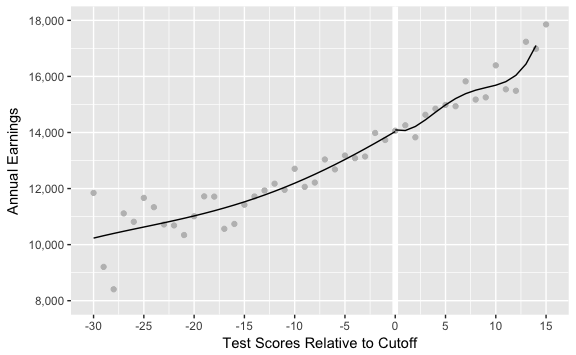
\includegraphics[width=0.7\linewidth]{sheepskin_files/figure-latex/fig.6.4-1} 

}

\caption{The effect of last-chance exam scores on earnings}(\#fig:fig.6.4)
\end{figure}

\hypertarget{references-9}{%
\section*{References}\label{references-9}}
\addcontentsline{toc}{section}{References}

\begin{itemize}
\tightlist
\item
  \url{http://masteringmetrics.com/wp-content/uploads/2015/02/ReadMe_Sheepskin.txt}
\item
  \url{http://masteringmetrics.com/wp-content/uploads/2015/02/cm_graphs.do}
\end{itemize}

\hypertarget{references-10}{%
\chapter*{References}\label{references-10}}
\addcontentsline{toc}{chapter}{References}

\hypertarget{refs}{}
\leavevmode\hypertarget{ref-AcemogluAngrist2000}{}%
Acemoglu, Daron, and Joshua Angrist. 2000. ``How Large Are Human-Capital
Externalities? Evidence from Compulsory Schooling Laws.'' \emph{NBER
Macroeconomics Annual}. \url{https://doi.org/10.1086/654403}.

\leavevmode\hypertarget{ref-Angrist2006}{}%
Angrist, Joshua D. 2006. ``Instrumental Variables Methods in
Experimental Criminological Research: What, Why and How.'' \emph{Journal
of Experimental Criminology}.
\url{https://doi.org/10.1007/s11292-005-5126-x}.

\leavevmode\hypertarget{ref-AngristKrueger1991}{}%
Angrist, Joshua D., and Alan B. Krueger. 1991. ``Does Compulsory School
Attendance Affect Schooling and Earnings?'' \emph{Quarterly Journal of
Economics}. \url{http://www.jstor.org/stable/2937954}.

\leavevmode\hypertarget{ref-AngristPischke2014}{}%
Angrist, Joshua D., and Jörn-Steffen Pischke. 2014. \emph{Mastering
'Metrics: The Path from Cause to Effect}. Princeton UP.
\url{https://press.princeton.edu/titles/10363.html}.

\leavevmode\hypertarget{ref-Aron-DineEinavEtAl2013}{}%
Aron-Dine, Aviva, Liran Einav, and Amy Finkelstein. 2013. ``The RAND
Health Insurance Experiment, Three Decades Later.'' \emph{Journal of
Economic Perspectives}. \url{https://doi.org/10.1257/jep.27.1.197}.

\leavevmode\hypertarget{ref-AshenfelterKrueger1994}{}%
Ashenfelter, Orley, and Alan Krueger. 1994. ``Estimates of the Economic
Return to Schooling from a New Sample of Twins.'' \emph{American
Economic Review}. \url{http://www.jstor.org/stable/2117766}.

\leavevmode\hypertarget{ref-AshenfelterRouse1998}{}%
Ashenfelter, Orley, and Cecilia Rouse. 1998. ``Income, Schooling, and
Ability: Evidence from a New Sample of Identical Twins.''
\emph{Quarterly Journal of Economics}.
\url{https://doi.org/10.1162/003355398555577}.

\leavevmode\hypertarget{ref-BrookWareEtAl1983}{}%
Brook, Robert H., Jr. John E. Ware, William H. Rogers, Emmett B. Keeler,
Allyson R. Davies, Cathy A. Donald, George A. Goldberg, Kathleen N.
Lohr, Patricia C. Masthay, and Joseph P. Newhouse. 1983. ``Does Free
Care Improve Adults' Health? --- Results from a Randomized Controlled
Trial.'' \emph{New England Journal of Medicine}.
\url{https://doi.org/10.1056/NEJM198312083092305}.

\leavevmode\hypertarget{ref-CarpenterDobkin2009}{}%
Carpenter, Christopher, and Carlos Dobkin. 2011. ``The Minimum Legal
Drinking Age and Public Health.'' \emph{Journal of Economic
Perspectives}. \url{https://doi.org/10.1257/jep.25.2.133}.

\leavevmode\hypertarget{ref-ClarkMartorell2014}{}%
Clark, Damon, and Paco Martorell. 2014. ``The Signaling Value of a High
School Diploma.'' \emph{Journal of Political Economy}.
\url{https://doi.org/10.1086/675238}.

\leavevmode\hypertarget{ref-DuMouchelWilliamsZador1987}{}%
Mouchel, William Du, Allan F. Williams, and Paul Zador. 1987. ``Raising
the Alcohol Purchase Age: Its Effects on Fatal Motor Vehicle Crashes in
Twenty-Six States.'' \emph{Journal of Legal Studies}.
\url{http://www.jstor.org/stable/724480}.

\leavevmode\hypertarget{ref-NorbergBierutGrucza2009}{}%
Norberg, Karen E., Laura J. Bierut, and Richard A. Grucza. 2009.
``Long-Term Effects of Minimum Drinking Age Laws on Past-Year Alcohol
and Drug Use Disorders.'' \emph{Alcoholism: Clinical and Experimental
Research}. \url{https://doi.org/10.1111/j.1530-0277.2009.01056.x}.

\leavevmode\hypertarget{ref-RichardsonTroost2009}{}%
Richardson, Gary, and William Troost. 2009. ``Monetary Intervention
Mitigated Banking Panics During the Great Depression: Quasi-Experimental
Evidence from a Federal Reserve District Border, 1929--1933.''
\emph{Journal of Political Economy}.
\url{https://doi.org/10.1086/649603}.

\leavevmode\hypertarget{ref-ShermanBerk1984}{}%
Sherman, Lawrence W., and Richard A. Berk. 1984. ``The Specific
Deterrent Effects of Arrest for Domestic Assault.'' \emph{American
Sociological Review}. \url{http://www.jstor.org/stable/2095575}.


\end{document}
